%\documentclass[conference]{IEEEtran}
\documentclass[nonacm,sigconf]{acmart}

%%
%% \BibTeX command to typeset BibTeX logo in the docs
%\AtBeginDocument{%
%  \providecommand\BibTeX{{%
%    Bib\TeX}}}

%\setcopyright{acmlicensed}
%\copyrightyear{2018}
%\acmYear{2018}
%\acmDOI{XXXXXXX.XXXXXXX}
%\acmConference[Conference acronym 'XX]{Make sure to enter the correct
%  conference title from your rights confirmation email}{June 03--05,
%  2018}{Woodstock, NY}
%\acmISBN{978-1-4503-XXXX-X/2018/06}


%\pagestyle{plain}
\usepackage{adjustbox}
\usepackage{float}
\usepackage{comment}
\usepackage{multirow}
\usepackage{array}
\usepackage{xspace}
\usepackage{color}
\usepackage{caption}
\usepackage{tabularx}
\usepackage{array}
\usepackage{ragged2e}
\usepackage{subcaption}
\usepackage{url}
\usepackage{graphicx}
\usepackage{enumitem}
\newcommand{\methodName}{RAM\xspace}
\newcommand{\asaf}[1]{\textbf{\color{blue}[[Asaf: #1]]}}
\newcommand{\new}[1]{\textcolor{red}{#1}}
\setcopyright{none}
\fancyfoot{}
% Some very useful LaTeX packages include:
% (uncomment the ones you want to load)

%\settopmatter{printacmref=false} % Removes citation information below abstract
\settopmatter{printacmref=false, printccs=false, printfolios=false}
\renewcommand\footnotetextcopyrightpermission[1]{} % Removes the ACM copyright footnot
%\acmConference[ ]{ }{ }{ }
%\acmBooktitle{}
%\acmPrice{}
%\acmISBN{}

\begin{document}
%
% paper title
% can use linebreaks \\ within to get better formatting as desired
\title{Rule-ATT\&CK Mapper (\methodName): Mapping SIEM Rules to TTPs Using LLMs}


% author names and affiliations
% use a multiple column layout for up to three different
% affiliations
\author{Prasanna N. Wudali}
\affiliation{%
  \institution{Ben-Gurion University of the Negev}
%  \city{City}
  \country{}
}

\author{Moshe Kravchik}
\affiliation{%
  \institution{Rafael Advanced Defense Systems}
%  \city{City}
  \country{}
}

\author{Ehud Malul, Parth A. Gandhi, Yuval Elovici, Asaf Shabtai}
\affiliation{%
  \institution{Ben-Gurion University of the Negev}
%  \city{City}
  \country{}
}
\renewcommand{\shortauthors}{}


\begin{abstract}
The growing frequency of cyberattacks has heightened the demand for accurate and efficient threat detection systems. 
Security information and event management (SIEM) platforms are important for analyzing log data and detecting adversarial activities through rule-based queries, also known as SIEM rules. 
The efficiency of the threat analysis process relies heavily on mapping these SIEM rules to the relevant attack techniques in the MITRE ATT\&CK framework. % is a critical step for making the threat analysis process efficient.
Inaccurate annotation of SIEM rules can result in the misinterpretation of attacks, increasing the likelihood that threats will be overlooked. 
Such misinterpretation can expose an organization's systems and networks to potential damage and security breaches.
Existing solutions for annotating SIEM rules with MITRE ATT\&CK technique and sub-technique labels have notable limitations: 
manual annotation of SIEM rules is both time-consuming and prone to errors, and machine learning-based approaches mainly focus on annotating unstructured free text sources (e.g., threat intelligence reports) rather than structured data like SIEM rules. 
Structured data often contains limited information, further complicating the annotation process and making it a challenging task.
To address these challenges, we propose Rule-ATT\&CK Mapper (\methodName), a novel framework that leverages large language models (LLMs) to automate the mapping of structured SIEM rules to MITRE ATT\&CK techniques. 
\methodName's multi-stage pipeline, which was inspired by the prompt chaining technique, enhances mapping accuracy without requiring LLM pretraining or fine-tuning. 
Using the Splunk Security Content dataset, we evaluate \methodName's performance using several LLMs, including GPT-4-Turbo, Qwen, IBM Granite, and Mistral. 
Our evaluation highlights GPT-4-Turbo’s superior performance, which derives from its enriched knowledge base, and an ablation study emphasizes the importance of external contextual knowledge in overcoming the limitations of LLMs' implicit knowledge for domain-specific tasks. 
These findings demonstrate \methodName's potential in automating cybersecurity workflows and provide valuable insights for future advancements in this field.

\end{abstract}

\keywords{SIEM rules, LLMs, MITRE ATT\&CK}

\maketitle

\thispagestyle{empty}


\section{\label{sec:intro}Introduction}


The rapid advancement of technology and widespread adoption of digital applications have resulted in a significant increase in cyberattacks~\cite{checkpoint}.
To gain visibility into their digital ecosystems, organizations deploy security information and event management (SIEM) systems in their networks. 
These systems store and analyze log data generated by various digital entities in the network~\cite{exabeam}.

SIEM systems enable threat detection by allowing users to execute search queries, referred to as rules, on the ingested log data. 
Each SIEM platform employs its own rule definition language (RDL), a schema-based structure for defining these rules that standardizes the creation and execution of SIEM rules, making them inherently structured data and a foundational component of modern cybersecurity operations.
Examples of such schemas include the search processing language (SPL) from Splunk, the Lucene query language by Elasticsearch, and the Kusto query language (KQL) by Microsoft. 

Security alerts are triggered when the execution of SIEM rules yields search results. 
When such alerts are generated, security analysts must examine each alert individually, performing tasks such as triage, analysis, and interpretation, and determine whether the alert corresponds to an actual attack. 
A critical aspect of effective threat detection and hunting is the precise mapping and understanding of the tactics, techniques, and procedures (TTPs) employed by adversaries, as defined in the MITRE ATT\&CK framework.\footnote{\url{https://attack.mitre.org/}} 
Incorporating MITRE ATT\&CK techniques in the analysis provides valuable insights, enabling analysts to discern potential attack flows. 
Such mapping enhances security professionals' ability to anticipate and mitigate the strategies employed by cyber adversaries.

Mapping SIEM rules to specific MITRE ATT\&CK techniques is a complex manual process that is prone to errors and can be time-consuming.
Cybero, a leading cybersecurity company, reported~\cite{cybero} that \textit{"organizations collect sufficient log data to potentially detect 94\% of techniques outlined in the MITRE ATT\&CK framework; however, only 24\% of these techniques are effectively covered due to gaps in detection rules, with an additional 12\% of SIEM rules rendered non-functional or misconfigured."} 
In its best practices guide~\cite{cisa} to MITRE ATT\&CK mapping, CISA, an American cyber defense agency, listed (i) leaping to conclusions (i.e., prematurely deciding on a mapping based on insufficient evidence or examination of the facts), (ii) missing opportunities (i.e., not considering, being unaware of, or overlooking other potential technique mappings based on implied or unclear information), and (iii) miscategorization (i.e., the selection of incorrect techniques due to misinterpreting, misreading, or inadequately understanding the techniques, specifically the difference between two techniques) as common mistakes committed by security analysts when manually performing the mapping task.
Given the above, there is a need to automate the mapping process and thereby reduce the workload on security analysts and increase the speed and accuracy of threat detection.

Recent cybersecurity research has explored various techniques for mapping unstructured data from cyber threat intelligence (CTI) reports to the MITRE ATT\&CK framework~\cite{alves2022leveraging,alam2023looking,rani2024ttpxhunter,liu2022threat,zhang2024attackgboosting}. 
While these methods have demonstrated effectiveness in handling unstructured data, they have a limited ability to adapt to structured data use cases, such as intrusion detection system and SIEM rules.
Also, these methods use supervised learning-based approaches to classify structured data (i.e., intrusion detection system and SIEM rules) to MITRE ATT\&CK technique classes, which require retraining when new threats emerge.
Their reliance on retraining limits their scalability and efficiency in dynamic threat landscapes.
Mărmureanu et al.~\cite{10398612} proposed a method to map structured data, specifically Splunk rules, to the MITRE ATT\&CK framework. 
This approach utilizes a BERT model trained as a classifier to categorize Splunk rules into 14 high-level MITRE ATT\&CK tactic classes. 
However, this method shares the same limitations as other supervised learning approaches discussed earlier, particularly the need for retraining with updated data to address new threats. 
Furthermore, the task of mapping rules to high-level tactics is comparatively easier than mapping them to MITRE ATT\&CK techniques and sub-techniques, which involve around 670 distinct classes and present a much greater challenge. 
Despite focusing on this simplified task, the method failed to achieve high performance in their evaluation, due to its inherent limitations.
In a recent study, Fayyazi et al.~\cite{fayyazi2023advancing} employed large language models (LLMs) to map CTIs in the form of unstructured text to MITRE ATT\&CK techniques, while Nir et al.~\cite{daniel2023labeling} employed them to map Snort intrusion detection rules to MITRE ATT\&CK techniques. 

These investigations highlight the potential of LLMs in cybersecurity tasks but also underscore their limitations. 
Solely relying on the implicit knowledge of LLMs has proven insufficient for addressing the domain-specific requirements of cybersecurity.
This gap highlights the need for more adaptable and scalable methodologies tailored to the dynamic nature of cyber threats.
To produce accurate and reliable predictions, they require additional contextual information that is not inherently available to the LLM.

To address these shortcomings, we propose \methodName, a novel LLM-based framework for analyzing SIEM rules and recommending relevant MITRE ATT\&CK techniques. 
\methodName eliminates dependence on training data, utilizes LLM agents to retrieve supplementary contextual information, and transforms structured rule into unstructured natural language to preserve the syntactic and semantic meaning of the rule.
This innovative approach ensures reliable and accurate predictions while overcoming the limitations of existing methods.

LLMs, with their advanced natural language processing (NLP) capabilities, can process and analyze structured data, automatically identify patterns, and understand the syntactic meaning of the data, but they often fall short in understanding the semantic meaning of the data.
This study leverages LLMs to autonomously map structured data in the form of SIEM rules %defined in any RDL 
to MITRE ATT\&CK techniques, enabling the automation of cybersecurity threat detection and investigation.

\methodName is a multi-stage AI agent pipeline (see Figure~\ref{fig:r2t}) inspired by the prompt chaining technique~\cite{wu2022promptchainer} and designed to enhance the understanding and application of SIEM rules. 
The pipeline begins with the extraction of indicators of compromise (IoCs) from the rule (e.g., process names, file names, registry keys and values, IP addresses, network ports).
Then, a web search LLM agent retrieves additional contextual information related to the IoCs identified in the rule. 
Leveraging the information gathered in the preceding stages, the next AI agent translates the rule into natural language text, providing a comprehensive description.
This textual description is then used by an LLM to identify the data source~\cite{ds} of the logs or the mitigation strategy being applied upon which the rule operates.
This natural language representation, along with the data source or mitigation-related information, serves as input to another LLM that maps the rule in question to probable MITRE ATT\&CK techniques. 
In the final stage, the pipeline refines the mapping and provides reasoning by extracting the most relevant techniques from the list of potential matches, facilitating precise alignment of the rule with the MITRE ATT\&CK framework.

We conducted a comprehensive series of experiments to evaluate \methodName's ability to map SIEM rules to the MITRE ATT\&CK framework. 
The evaluation focused on common metrics such as precision and recall, which are indicators of the method's accuracy and completeness in correctly classifying the SIEM rules to relevant techniques within the framework.
Various LLMs were examined, including Qwen, IBM Granite, Mistral, and GPT-4-Turbo, and we evaluated \methodName's effectiveness when each LLM was employed in the pipeline.
We used the threat detection rules published in the Splunk Security content dataset\footnote{\url{https://github.com/splunk/security_content/tree/develop/detections}} in our experiments; to ensure that the rules were not already known to the LLM, we carefully selected rules for the dataset based on their creation or modification dates. 
Specifically, we included only those rules with dates later than the knowledge cut-off date of the LLMs utilized in our experiments. 


Using various configuration settings, we aimed to identify the optimal strategies for maximizing the performance of these models. 
Our study not only demonstrates the potential of LLMs in automating threat analysis but also provides insights into the most effective configurations for deploying these models in real-world cybersecurity environments. 
This study is among the first to explore leveraging LLMs to map structured data to the MITRE ATT\&CK framework, and our results, which highlight RAM's potential, leave room for further refinement in future research. 
We also provide valuable insights regarding the challenges encountered during this study, which can guide subsequent advancements in this domain for example, the lack of a completely labeled SIEM rules dataset.

\noindent The main contributions of this paper are as follows:

\begin{itemize}[nosep,leftmargin=*]
    \item We demonstrate the feasibility of using LLMs to automate the mapping of SIEM rules to MITRE ATT\&CK techniques and provide reasoning, which could significantly enhance the capabilities of current cybersecurity tools.
    \item We propose an AI agent-based framework that utilizes both implicit and explicit knowledge in automating the mapping of structured SIEM rules to MITRE ATT\&CK techniques.
    \item We demonstrate the effective utilization of LLMs without the need for pretraining or fine-tuning, thereby eliminating the need for any training data.
    \item We provide a practical guide for deploying LLMs in cybersecurity, by identifying the optimal configurations for these models.
   
    \item We present valuable insights regarding the challenges encountered during the experimentation process, providing increased understanding of the obstacles and considerations that shaped our research and findings.
\end{itemize}


\begin{figure*}[ht!]
    \centering
    \includegraphics[width=0.85\linewidth]{Images/r2t_method_new.jpg}
    \caption{Overview of our AI Agent-based \methodName pipeline.}
    \label{fig:r2t}
\end{figure*}
\section{Background}\label{sec:backgrnd}

\subsection{Cold Start Latency and Mitigation Techniques}

Traditional FaaS platforms mitigate cold starts through snapshotting, lightweight virtualization, and warm-state management. Snapshot-based methods like \textbf{REAP} and \textbf{Catalyzer} reduce initialization time by preloading or restoring container states but require significant memory and I/O resources, limiting scalability~\cite{dong_catalyzer_2020, ustiugov_benchmarking_2021}. Lightweight virtualization solutions, such as \textbf{Firecracker} microVMs, achieve fast startup times with strong isolation but depend on robust infrastructure, making them less adaptable to fluctuating workloads~\cite{agache_firecracker_2020}. Warm-state management techniques like \textbf{Faa\$T}~\cite{romero_faa_2021} and \textbf{Kraken}~\cite{vivek_kraken_2021} keep frequently invoked containers ready, balancing readiness and cost efficiency under predictable workloads but incurring overhead when demand is erratic~\cite{romero_faa_2021, vivek_kraken_2021}. While these methods perform well in resource-rich cloud environments, their resource intensity challenges applicability in edge settings.

\subsubsection{Edge FaaS Perspective}

In edge environments, cold start mitigation emphasizes lightweight designs, resource sharing, and hybrid task distribution. Lightweight execution environments like unikernels~\cite{edward_sock_2018} and \textbf{Firecracker}~\cite{agache_firecracker_2020}, as used by \textbf{TinyFaaS}~\cite{pfandzelter_tinyfaas_2020}, minimize resource usage and initialization delays but require careful orchestration to avoid resource contention. Function co-location, demonstrated by \textbf{Photons}~\cite{v_dukic_photons_2020}, reduces redundant initializations by sharing runtime resources among related functions, though this complicates isolation in multi-tenant setups~\cite{v_dukic_photons_2020}. Hybrid offloading frameworks like \textbf{GeoFaaS}~\cite{malekabbasi_geofaas_2024} balance edge-cloud workloads by offloading latency-tolerant tasks to the cloud and reserving edge resources for real-time operations, requiring reliable connectivity and efficient task management. These edge-specific strategies address cold starts effectively but introduce challenges in scalability and orchestration.

\subsection{Predictive Scaling and Caching Techniques}

Efficient resource allocation is vital for maintaining low latency and high availability in serverless platforms. Predictive scaling and caching techniques dynamically provision resources and reduce cold start latency by leveraging workload prediction and state retention.
Traditional FaaS platforms use predictive scaling and caching to optimize resources, employing techniques (OFC, FaasCache) to reduce cold starts. However, these methods rely on centralized orchestration and workload predictability, limiting their effectiveness in dynamic, resource-constrained edge environments.



\subsubsection{Edge FaaS Perspective}

Edge FaaS platforms adapt predictive scaling and caching techniques to constrain resources and heterogeneous environments. \textbf{EDGE-Cache}~\cite{kim_delay-aware_2022} uses traffic profiling to selectively retain high-priority functions, reducing memory overhead while maintaining readiness for frequent requests. Hybrid frameworks like \textbf{GeoFaaS}~\cite{malekabbasi_geofaas_2024} implement distributed caching to balance resources between edge and cloud nodes, enabling low-latency processing for critical tasks while offloading less critical workloads. Machine learning methods, such as clustering-based workload predictors~\cite{gao_machine_2020} and GRU-based models~\cite{guo_applying_2018}, enhance resource provisioning in edge systems by efficiently forecasting workload spikes. These innovations effectively address cold start challenges in edge environments, though their dependency on accurate predictions and robust orchestration poses scalability challenges.

\subsection{Decentralized Orchestration, Function Placement, and Scheduling}

Efficient orchestration in serverless platforms involves workload distribution, resource optimization, and performance assurance. While traditional FaaS platforms rely on centralized control, edge environments require decentralized and adaptive strategies to address unique challenges such as resource constraints and heterogeneous hardware.



\subsubsection{Edge FaaS Perspective}

Edge FaaS platforms adopt decentralized and adaptive orchestration frameworks to meet the demands of resource-constrained environments. Systems like \textbf{Wukong} distribute scheduling across edge nodes, enhancing data locality and scalability while reducing network latency. Lightweight frameworks such as \textbf{OpenWhisk Lite}~\cite{kravchenko_kpavelopenwhisk-light_2024} optimize resource allocation by decentralizing scheduling policies, minimizing cold starts and latency in edge setups~\cite{benjamin_wukong_2020}. Hybrid solutions like \textbf{OpenFaaS}~\cite{noauthor_openfaasfaas_2024} and \textbf{EdgeMatrix}~\cite{shen_edgematrix_2023} combine edge-cloud orchestration to balance resource utilization, retaining latency-sensitive functions at the edge while offloading non-critical workloads to the cloud. While these approaches improve flexibility, they face challenges in maintaining coordination and ensuring consistent performance across distributed nodes.


\section{Related Works}
\label{sec:related_works}


\noindent\textbf{Diffusion-based Video Generation. }
The advancement of diffusion models \cite{rombach2022high, ramesh2022hierarchical, zheng2022entropy} has led to significant progress in video generation. Due to the scarcity of high-quality video-text datasets \cite{Blattmann2023, Blattmann2023a}, researchers have adapted existing text-to-image (T2I) models to facilitate text-to-video (T2V) generation. Notable examples include AnimateDiff \cite{Guo2023}, Align your Latents \cite{Blattmann2023a}, PYoCo \cite{ge2023preserve}, and Emu Video \cite{girdhar2023emu}. Further advancements, such as LVDM \cite{he2022latent}, VideoCrafter \cite{chen2023videocrafter1, chen2024videocrafter2}, ModelScope \cite{wang2023modelscope}, LAVIE \cite{wang2023lavie}, and VideoFactory \cite{wang2024videofactory}, have refined these approaches by fine-tuning both spatial and temporal blocks, leveraging T2I models for initialization to improve video quality.
Recently, Sora \cite{brooks2024video} and CogVideoX \cite{yang2024cogvideox} enhance video generation by introducing Transformer-based diffusion backbones \cite{Peebles2023, Ma2024, Yu2024} and utilizing 3D-VAE, unlocking the potential for realistic world simulators. Additionally, SVD \cite{Blattmann2023}, SEINE \cite{chen2023seine}, PixelDance \cite{zeng2024make} and PIA \cite{zhang2024pia} have made significant strides in image-to-video generation, achieving notable improvements in quality and flexibility.
Further, I2VGen-XL \cite{zhang2023i2vgen}, DynamicCrafter \cite{Xing2023}, and Moonshot \cite{zhang2024moonshot} incorporate additional cross-attention layers to strengthen conditional signals during generation.



\noindent\textbf{Controllable Generation.}
Controllable generation has become a central focus in both image \citep{Zhang2023,jiang2024survey, Mou2024, Zheng2023, peng2024controlnext, ye2023ip, wu2024spherediffusion, song2024moma, wu2024ifadapter} and video \citep{gong2024atomovideo, zhang2024moonshot, guo2025sparsectrl, jiang2024videobooth} generation, enabling users to direct the output through various types of control. A wide range of controllable inputs has been explored, including text descriptions, pose \citep{ma2024follow,wang2023disco,hu2024animate,xu2024magicanimate}, audio \citep{tang2023anytoany,tian2024emo,he2024co}, identity representations \citep{chefer2024still,wang2024customvideo,wu2024customcrafter}, trajectory \citep{yin2023dragnuwa,chen2024motion,li2024generative,wu2024motionbooth, namekata2024sg}.


\noindent\textbf{Text-based Camera Control.}
Text-based camera control methods use natural language descriptions to guide camera motion in video generation. AnimateDiff \cite{Guo2023} and SVD \cite{Blattmann2023} fine-tune LoRAs \cite{hu2021lora} for specific camera movements based on text input. 
Image conductor\cite{li2024image} proposed to separate different camera and object motions through camera LoRA weight and object LoRA weight to achieve more precise motion control.
In contrast, MotionMaster \cite{hu2024motionmaster} and Peekaboo \cite{jain2024peekaboo} offer training-free approaches for generating coarse-grained camera motions, though with limited precision. VideoComposer \cite{wang2024videocomposer} adjusts pixel-level motion vectors to provide finer control, but challenges remain in achieving precise camera control.

\noindent\textbf{Trajectory-based Camera Control.}
MotionCtrl \cite{Wang2024Motionctrl}, CameraCtrl \cite{He2024Cameractrl}, and Direct-a-Video \cite{yang2024direct} use camera pose as input to enhance control, while CVD \cite{kuang2024collaborative} extends CameraCtrl for multi-view generation, though still limited by motion complexity. To improve geometric consistency, Pose-guided diffusion \cite{tseng2023consistent}, CamCo \cite{Xu2024}, and CamI2V \cite{zheng2024cami2v} apply epipolar constraints for consistent viewpoints. VD3D \cite{bahmani2024vd3d} introduces a ControlNet\cite{Zhang2023}-like conditioning mechanism with spatiotemporal camera embeddings, enabling more precise control.
CamTrol \cite{hou2024training} offers a training-free approach that renders static point clouds into multi-view frames for video generation. Cavia \cite{xu2024cavia} introduces view-integrated attention mechanisms to improve viewpoint and temporal consistency, while I2VControl-Camera \cite{feng2024i2vcontrol} refines camera movement by employing point trajectories in the camera coordinate system. Despite these advancements, challenges in maintaining camera control and scene-scale consistency remain, which our method seeks to address. It is noted that 4Dim~\cite{watson2024controlling} introduces absolute scale but in  4D novel view synthesis (NVS) of scenes.



\section{Research Methodology}~\label{sec:Methodology}

In this section, we discuss the process of conducting our systematic review, e.g., our search strategy for data extraction of relevant studies, based on the guidelines of Kitchenham et al.~\cite{kitchenham2022segress} to conduct SLRs and Petersen et al.~\cite{PETERSEN20151} to conduct systematic mapping studies (SMSs) in Software Engineering. In this systematic review, we divide our work into a four-stage procedure, including planning, conducting, building a taxonomy, and reporting the review, illustrated in Fig.~\ref{fig:search}. The four stages are as follows: (1) the \emph{planning} stage involved identifying research questions (RQs) and specifying the detailed research plan for the study; (2) the \emph{conducting} stage involved analyzing and synthesizing the existing primary studies to answer the research questions; (3) the \emph{taxonomy} stage was introduced to optimize the data extraction results and consolidate a taxonomy schema for REDAST methodology; (4) the \emph{reporting} stage involved the reviewing, concluding and reporting the final result of our study.

\begin{figure}[!t]
    \centering
    \includegraphics[width=1\linewidth]{fig/methodology/searching-process.drawio.pdf}
    \caption{Systematic Literature Review Process}
    \label{fig:search}
\end{figure}

\subsection{Research Questions}
In this study, we developed five research questions (RQs) to identify the input and output, analyze technologies, evaluate metrics, identify challenges, and identify potential opportunities. 

\textbf{RQ1. What are the input configurations, formats, and notations used in the requirements in requirements-driven
automated software testing?} In requirements-driven testing, the input is some form of requirements specification -- which can vary significantly. RQ1 maps the input for REDAST and reports on the comparison among different formats for requirements specification.

\textbf{RQ2. What are the frameworks, tools, processing methods, and transformation techniques used in requirements-driven automated software testing studies?} RQ2 explores the technical solutions from requirements to generated artifacts, e.g., rule-based transformation applying natural language processing (NLP) pipelines and deep learning (DL) techniques, where we additionally discuss the potential intermediate representation and additional input for the transformation process.

\textbf{RQ3. What are the test formats and coverage criteria used in the requirements-driven automated software
testing process?} RQ3 focuses on identifying the formulation of generated artifacts (i.e., the final output). We map the adopted test formats and analyze their characteristics in the REDAST process.

\textbf{RQ4. How do existing studies evaluate the generated test artifacts in the requirements-driven automated software testing process?} RQ4 identifies the evaluation datasets, metrics, and case study methodologies in the selected papers. This aims to understand how researchers assess the effectiveness, accuracy, and practical applicability of the generated test artifacts.

\textbf{RQ5. What are the limitations and challenges of existing requirements-driven automated software testing methods in the current era?} RQ5 addresses the limitations and challenges of existing studies while exploring future directions in the current era of technology development. %It particularly highlights the potential benefits of advanced LLMs and examines their capacity to meet the high expectations placed on these cutting-edge language modeling technologies. %\textcolor{blue}{CA: Do we really need to focus on LLMs? TBD.} \textcolor{orange}{FW: About LLMs, I removed the direct emphase in RQ5 but kept the discussion in RQ5 and the solution section. I think that would be more appropriate.}

\subsection{Searching Strategy}

The overview of the search process is exhibited in Fig. \ref{fig:papers}, which includes all the details of our search steps.
\begin{table}[!ht]
\caption{List of Search Terms}
\label{table:search_term}
\begin{tabularx}{\textwidth}{lX}
\hline
\textbf{Terms Group} & \textbf{Terms} \\ \hline
Test Group & test* \\
Requirement Group & requirement* OR use case* OR user stor* OR specification* \\
Software Group & software* OR system* \\
Method Group & generat* OR deriv* OR map* OR creat* OR extract* OR design* OR priorit* OR construct* OR transform* \\ \hline
\end{tabularx}
\end{table}

\begin{figure}
    \centering
    \includegraphics[width=1\linewidth]{fig/methodology/search-papers.drawio.pdf}
    \caption{Study Search Process}
    \label{fig:papers}
\end{figure}

\subsubsection{Search String Formulation}
Our research questions (RQs) guided the identification of the main search terms. We designed our search string with generic keywords to avoid missing out on any related papers, where four groups of search terms are included, namely ``test group'', ``requirement group'', ``software group'', and ``method group''. In order to capture all the expressions of the search terms, we use wildcards to match the appendix of the word, e.g., ``test*'' can capture ``testing'', ``tests'' and so on. The search terms are listed in Table~\ref{table:search_term}, decided after iterative discussion and refinement among all the authors. As a result, we finally formed the search string as follows:


\hangindent=1.5em
 \textbf{ON ABSTRACT} ((``test*'') \textbf{AND} (``requirement*'' \textbf{OR} ``use case*'' \textbf{OR} ``user stor*'' \textbf{OR} ``specifications'') \textbf{AND} (``software*'' \textbf{OR} ``system*'') \textbf{AND} (``generat*'' \textbf{OR} ``deriv*'' \textbf{OR} ``map*'' \textbf{OR} ``creat*'' \textbf{OR} ``extract*'' \textbf{OR} ``design*'' \textbf{OR} ``priorit*'' \textbf{OR} ``construct*'' \textbf{OR} ``transform*''))

The search process was conducted in September 2024, and therefore, the search results reflect studies available up to that date. We conducted the search process on six online databases: IEEE Xplore, ACM Digital Library, Wiley, Scopus, Web of Science, and Science Direct. However, some databases were incompatible with our default search string in the following situations: (1) unsupported for searching within abstract, such as Scopus, and (2) limited search terms, such as ScienceDirect. Here, for (1) situation, we searched within the title, keyword, and abstract, and for (2) situation, we separately executed the search and removed the duplicate papers in the merging process. 

\subsubsection{Automated Searching and Duplicate Removal}
We used advanced search to execute our search string within our selected databases, following our designed selection criteria in Table \ref{table:selection}. The first search returned 27,333 papers. Specifically for the duplicate removal, we used a Python script to remove (1) overlapped search results among multiple databases and (2) conference or workshop papers, also found with the same title and authors in the other journals. After duplicate removal, we obtained 21,652 papers for further filtering.

\begin{table*}[]
\caption{Selection Criteria}
\label{table:selection}
\begin{tabularx}{\textwidth}{lX}
\hline
\textbf{Criterion ID} & \textbf{Criterion Description} \\ \hline
S01          & Papers written in English. \\
S02-1        & Papers in the subjects of "Computer Science" or "Software Engineering". \\
S02-2        & Papers published on software testing-related issues. \\
S03          & Papers published from 1991 to the present. \\ 
S04          & Papers with accessible full text. \\ \hline
\end{tabularx}
\end{table*}

\begin{table*}[]
\small
\caption{Inclusion and Exclusion Criteria}
\label{table:criteria}
\begin{tabularx}{\textwidth}{lX}
\hline
\textbf{ID}  & \textbf{Description} \\ \hline
\multicolumn{2}{l}{\textbf{Inclusion Criteria}} \\ \hline
I01 & Papers about requirements-driven automated system testing or acceptance testing generation, or studies that generate system-testing-related artifacts. \\
I02 & Peer-reviewed studies that have been used in academia with references from literature. \\ \hline
\multicolumn{2}{l}{\textbf{Exclusion Criteria}} \\ \hline
E01 & Studies that only support automated code generation, but not test-artifact generation. \\
E02 & Studies that do not use requirements-related information as an input. \\
E03 & Papers with fewer than 5 pages (1-4 pages). \\
E04 & Non-primary studies (secondary or tertiary studies). \\
E05 & Vision papers and grey literature (unpublished work), books (chapters), posters, discussions, opinions, keynotes, magazine articles, experience, and comparison papers. \\ \hline
\end{tabularx}
\end{table*}

\subsubsection{Filtering Process}

In this step, we filtered a total of 21,652 papers using the inclusion and exclusion criteria outlined in Table \ref{table:criteria}. This process was primarily carried out by the first and second authors. Our criteria are structured at different levels, facilitating a multi-step filtering process. This approach involves applying various criteria in three distinct phases. We employed a cross-verification method involving (1) the first and second authors and (2) the other authors. Initially, the filtering was conducted separately by the first and second authors. After cross-verifying their results, the results were then reviewed and discussed further by the other authors for final decision-making. We widely adopted this verification strategy within the filtering stages. During the filtering process, we managed our paper list using a BibTeX file and categorized the papers with color-coding through BibTeX management software\footnote{\url{https://bibdesk.sourceforge.io/}}, i.e., “red” for irrelevant papers, “yellow” for potentially relevant papers, and “blue” for relevant papers. This color-coding system facilitated the organization and review of papers according to their relevance.

The screening process is shown below,
\begin{itemize}
    \item \textbf{1st-round Filtering} was based on the title and abstract, using the criteria I01 and E01. At this stage, the number of papers was reduced from 21,652 to 9,071.
    \item \textbf{2nd-round Filtering}. We attempted to include requirements-related papers based on E02 on the title and abstract level, which resulted from 9,071 to 4,071 papers. We excluded all the papers that did not focus on requirements-related information as an input or only mentioned the term ``requirements'' but did not refer to the requirements specification.
    \item \textbf{3rd-round Filtering}. We selectively reviewed the content of papers identified as potentially relevant to requirements-driven automated test generation. This process resulted in 162 papers for further analysis.
\end{itemize}
Note that, especially for third-round filtering, we aimed to include as many relevant papers as possible, even borderline cases, according to our criteria. The results were then discussed iteratively among all the authors to reach a consensus.

\subsubsection{Snowballing}

Snowballing is necessary for identifying papers that may have been missed during the automated search. Following the guidelines by Wohlin~\cite{wohlin2014guidelines}, we conducted both forward and backward snowballing. As a result, we identified 24 additional papers through this process.

\subsubsection{Data Extraction}

Based on the formulated research questions (RQs), we designed 38 data extraction questions\footnote{\url{https://drive.google.com/file/d/1yjy-59Juu9L3WHaOPu-XQo-j-HHGTbx_/view?usp=sharing}} and created a Google Form to collect the required information from the relevant papers. The questions included 30 short-answer questions, six checkbox questions, and two selection questions. The data extraction was organized into five sections: (1) basic information: fundamental details such as title, author, venue, etc.; (2) open information: insights on motivation, limitations, challenges, etc.; (3) requirements: requirements format, notation, and related aspects; (4) methodology: details, including immediate representation and technique support; (5) test-related information: test format(s), coverage, and related elements. Similar to the filtering process, the first and second authors conducted the data extraction and then forwarded the results to the other authors to initiate the review meeting.

\subsubsection{Quality Assessment}

During the data extraction process, we encountered papers with insufficient information. To address this, we conducted a quality assessment in parallel to ensure the relevance of the papers to our objectives. This approach, also adopted in previous secondary studies~\cite{shamsujjoha2021developing, naveed2024model}, involved designing a set of assessment questions based on guidelines by Kitchenham et al.~\cite{kitchenham2022segress}. The quality assessment questions in our study are shown below:
\begin{itemize}
    \item \textbf{QA1}. Does this study clearly state \emph{how} requirements drive automated test generation?
    \item \textbf{QA2}. Does this study clearly state the \emph{aim} of REDAST?
    \item \textbf{QA3}. Does this study enable \emph{automation} in test generation?
    \item \textbf{QA4}. Does this study demonstrate the usability of the method from the perspective of methodology explanation, discussion, case examples, and experiments?
\end{itemize}
QA4 originates from an open perspective in the review process, where we focused on evaluation, discussion, and explanation. Our review also examined the study’s overall structure, including the methodology description, case studies, experiments, and analyses. The detailed results of the quality assessment are provided in the Appendix. Following this assessment, the final data extraction was based on 156 papers.

% \begin{table}[]
% \begin{tabular}{ll}
% \hline
% QA ID & QA Questions                                             \\ \hline
% Q01   & Does this study clearly state its aims?                  \\
% Q02   & Does this study clearly describe its methodology?        \\
% Q03   & Does this study involve automated test generation?       \\
% Q04   & Does this study include a promising evaluation?          \\
% Q05   & Does this study demonstrate the usability of the method? \\ \hline
% \end{tabular}%
% \caption{Questions for Quality Assessment}
% \label{table:qa}
% \end{table}

% automated quality assessment

% \textcolor{blue}{CA: Our search strategy focused on identifying requirements types first. We covered several sources, e.g., ~\cite{Pohl:11,wagner2019status} to identify different formats and notations of specifying requirements. However, this came out to be a long list, e.g., free-form NL requirements, semi-formal UML models, free-from textual use case models, UML class diagrams, UML activity diagrams, and so on. In this paper, we attempted to primarily focus on requirements-related aspects and not design-level information. Hence, we generalised our search string to include generic keywords, e.g., requirement*, use case*, and user stor*. We did so to avoid missing out on any papers, bringing too restrictive in our search strategy, and not creating a too-generic search string with all the aforementioned formats to avoid getting results beyond our review's scope.}


%% Use \subsection commands to start a subsection.



%\subsection{Study Selection}

% In this step, we further looked into the content of searched papers using our search strategy and applied our inclusion and exclusion criteria. Our filtering strategy aimed to pinpoint studies focused on requirements-driven system-level testing. Recognizing the presence of irrelevant papers in our search results, we established detailed selection criteria for preliminary inclusion and exclusion, as shown in Table \ref{table: criteria}. Specifically, we further developed the taxonomy schema to exclude two types of studies that did not meet the requirements for system-level testing: (1) studies supporting specification-driven test generation, such as UML-driven test generation, rather than requirements-driven testing, and (2) studies focusing on code-based test generation, such as requirement-driven code generation for unit testing.




\definecolor{darkgreen}{rgb}{0.0, 0.5, 0.0}
\definecolor{violet}{rgb}{0.56, 0.0, 1.0}
\section{Evaluation}
We apply our methodology to derive counterfactual policies for various MDPs, addressing three main research questions: (1) how does our policy's performance compare to the Gumbel-max SCM approach; (2) how do the counterfactual stability and monotonicity assumptions impact the probability bounds; and (3) how fast is our approach compared with the Gumbel-max SCM method?

\begin{figure*}
    \centering
    %
    \resizebox{0.6\textwidth}{!}{
        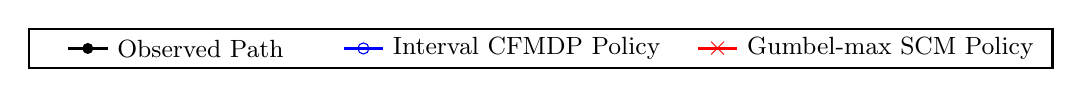
\begin{tikzpicture}[scale=1.0, every node/.style={scale=1.0}]
            \draw[thick, black] (-3, -0.25) rectangle (10, 0.25);
            %
            \draw[black, line width=1pt] (-2.5, 0.0) -- (-2,0.0);
            \fill[black] (-2.25,0.0) circle (2pt); %
            \node[right] at (-2,0.0) {\small Observed Path};
            
            %
            \draw[blue, line width=1pt] (1.0,0.0) -- (1.5,0.0);
            \node[draw=blue, circle, minimum size=4pt, inner sep=0pt] at (1.25,0.0) {}; %
            \node[right] at (1.5,0.0) {\small Interval CFMDP Policy};
            
            %
            \draw[red, line width=1pt] (5.5,0) -- (6,0);
            \node[red] at (5.75,0) {$\boldsymbol{\times}$}; %
            \node[right] at (6,0) {\small Gumbel-max SCM Policy};
        \end{tikzpicture}
    }\\
    %
    \subfigure[\footnotesize Lowest cumulative reward: Interval CFMDP ($312$), Gumbel-max SCM ($312$)]{%
        \resizebox{0.76\columnwidth}{!}{
             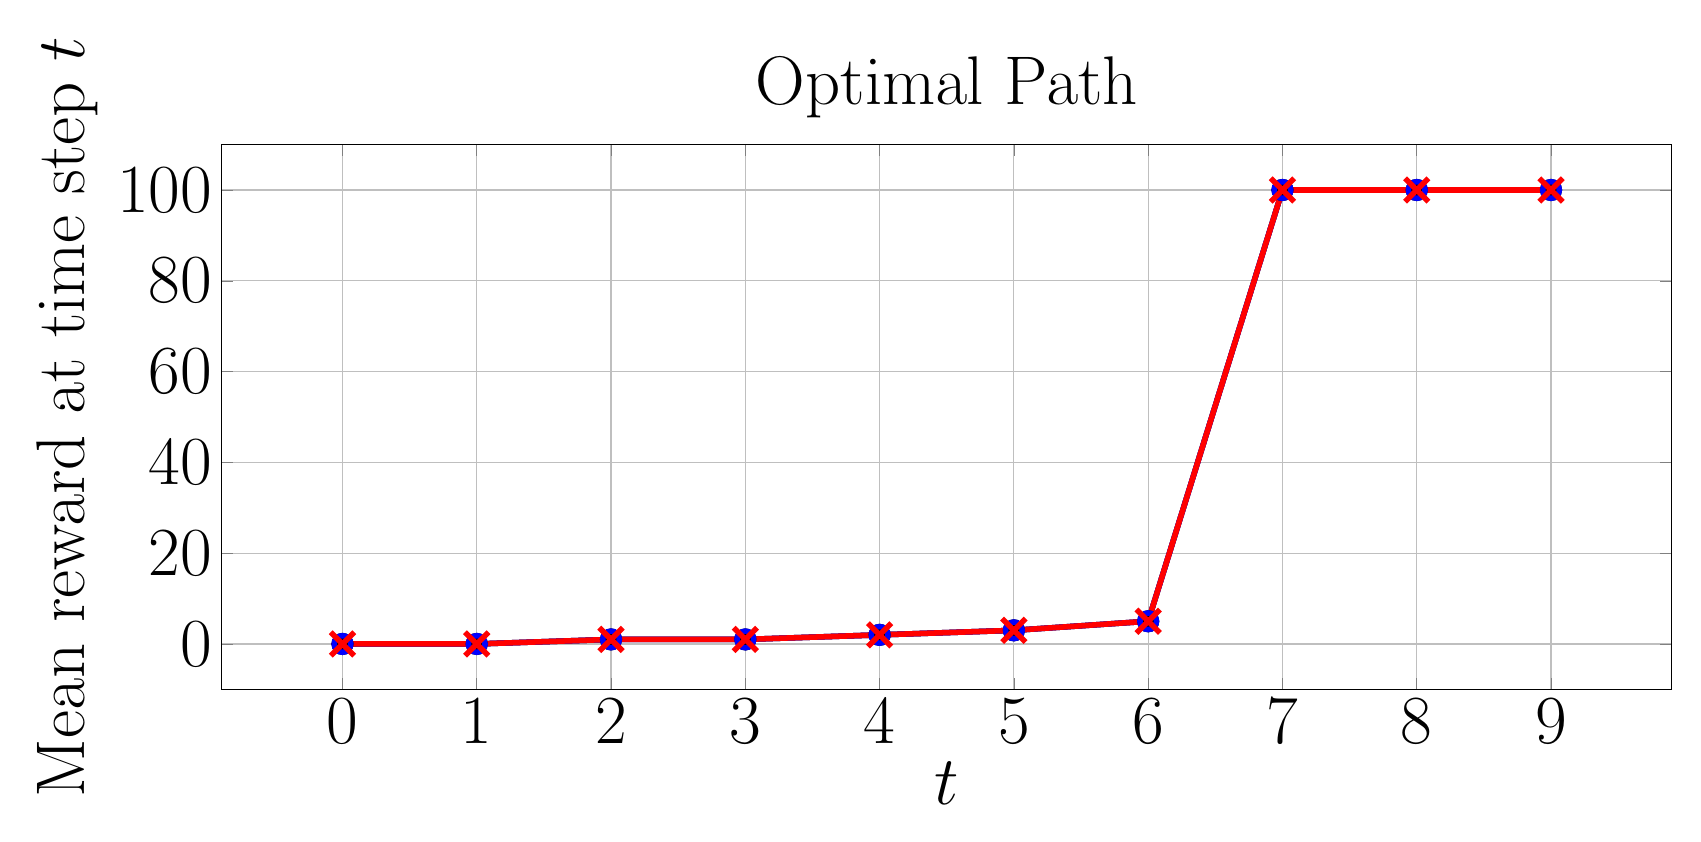
\begin{tikzpicture}
                \begin{axis}[
                    xlabel={$t$},
                    ylabel={Mean reward at time step $t$},
                    title={Optimal Path},
                    grid=both,
                    width=20cm, height=8.5cm,
                    every axis/.style={font=\Huge},
                    %
                ]
                \addplot[
                    color=black, %
                    mark=*, %
                    line width=2pt,
                    mark size=3pt,
                    error bars/.cd,
                    y dir=both, %
                    y explicit, %
                    error bar style={line width=1pt,solid},
                    error mark options={line width=1pt,mark size=4pt,rotate=90}
                ]
                coordinates {
                    (0, 0.0)  +- (0, 0.0)
                    (1, 0.0)  +- (0, 0.0) 
                    (2, 1.0)  +- (0, 0.0) 
                    (3, 1.0)  +- (0, 0.0)
                    (4, 2.0)  +- (0, 0.0)
                    (5, 3.0) +- (0, 0.0)
                    (6, 5.0) +- (0, 0.0)
                    (7, 100.0) +- (0, 0.0)
                    (8, 100.0) +- (0, 0.0)
                    (9, 100.0) +- (0, 0.0)
                };
                %
                \addplot[
                    color=blue, %
                    mark=o, %
                    line width=2pt,
                    mark size=3pt,
                    error bars/.cd,
                    y dir=both, %
                    y explicit, %
                    error bar style={line width=1pt,solid},
                    error mark options={line width=1pt,mark size=4pt,rotate=90}
                ]
                 coordinates {
                    (0, 0.0)  +- (0, 0.0)
                    (1, 0.0)  +- (0, 0.0) 
                    (2, 1.0)  +- (0, 0.0) 
                    (3, 1.0)  +- (0, 0.0)
                    (4, 2.0)  +- (0, 0.0)
                    (5, 3.0) +- (0, 0.0)
                    (6, 5.0) +- (0, 0.0)
                    (7, 100.0) +- (0, 0.0)
                    (8, 100.0) +- (0, 0.0)
                    (9, 100.0) +- (0, 0.0)
                };
                %
                \addplot[
                    color=red, %
                    mark=x, %
                    line width=2pt,
                    mark size=6pt,
                    error bars/.cd,
                    y dir=both, %
                    y explicit, %
                    error bar style={line width=1pt,solid},
                    error mark options={line width=1pt,mark size=4pt,rotate=90}
                ]
                coordinates {
                    (0, 0.0)  +- (0, 0.0)
                    (1, 0.0)  +- (0, 0.0) 
                    (2, 1.0)  +- (0, 0.0) 
                    (3, 1.0)  +- (0, 0.0)
                    (4, 2.0)  +- (0, 0.0)
                    (5, 3.0) +- (0, 0.0)
                    (6, 5.0) +- (0, 0.0)
                    (7, 100.0) +- (0, 0.0)
                    (8, 100.0) +- (0, 0.0)
                    (9, 100.0) +- (0, 0.0)
                };
                \end{axis}
            \end{tikzpicture}
         }
    }
    \hspace{1cm}
    \subfigure[\footnotesize Lowest cumulative reward: Interval CFMDP ($19$), Gumbel-max SCM ($-88$)]{%
         \resizebox{0.76\columnwidth}{!}{
            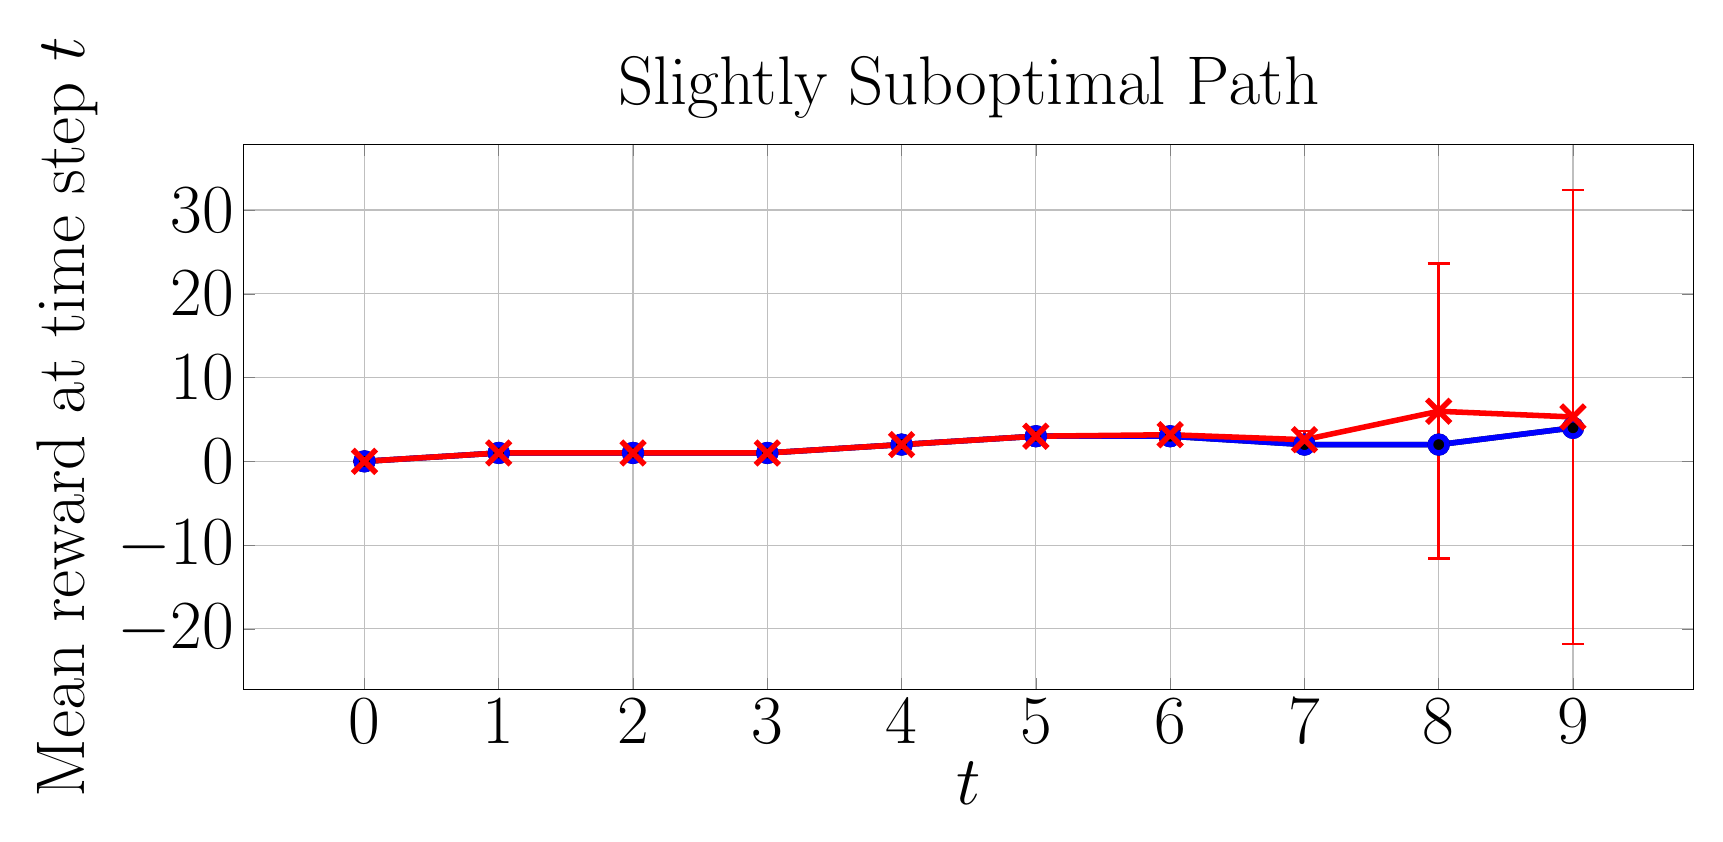
\begin{tikzpicture}
                \begin{axis}[
                    xlabel={$t$},
                    ylabel={Mean reward at time step $t$},
                    title={Slightly Suboptimal Path},
                    grid=both,
                    width=20cm, height=8.5cm,
                    every axis/.style={font=\Huge},
                    %
                ]
                \addplot[
                    color=black, %
                    mark=*, %
                    line width=2pt,
                    mark size=3pt,
                    error bars/.cd,
                    y dir=both, %
                    y explicit, %
                    error bar style={line width=1pt,solid},
                    error mark options={line width=1pt,mark size=4pt,rotate=90}
                ]
              coordinates {
                    (0, 0.0)  +- (0, 0.0)
                    (1, 1.0)  +- (0, 0.0) 
                    (2, 1.0)  +- (0, 0.0) 
                    (3, 1.0)  +- (0, 0.0)
                    (4, 2.0)  +- (0, 0.0)
                    (5, 3.0) +- (0, 0.0)
                    (6, 3.0) +- (0, 0.0)
                    (7, 2.0) +- (0, 0.0)
                    (8, 2.0) +- (0, 0.0)
                    (9, 4.0) +- (0, 0.0)
                };
                %
                \addplot[
                    color=blue, %
                    mark=o, %
                    line width=2pt,
                    mark size=3pt,
                    error bars/.cd,
                    y dir=both, %
                    y explicit, %
                    error bar style={line width=1pt,solid},
                    error mark options={line width=1pt,mark size=4pt,rotate=90}
                ]
              coordinates {
                    (0, 0.0)  +- (0, 0.0)
                    (1, 1.0)  +- (0, 0.0) 
                    (2, 1.0)  +- (0, 0.0) 
                    (3, 1.0)  +- (0, 0.0)
                    (4, 2.0)  +- (0, 0.0)
                    (5, 3.0) +- (0, 0.0)
                    (6, 3.0) +- (0, 0.0)
                    (7, 2.0) +- (0, 0.0)
                    (8, 2.0) +- (0, 0.0)
                    (9, 4.0) +- (0, 0.0)
                };
                %
                \addplot[
                    color=red, %
                    mark=x, %
                    line width=2pt,
                    mark size=6pt,
                    error bars/.cd,
                    y dir=both, %
                    y explicit, %
                    error bar style={line width=1pt,solid},
                    error mark options={line width=1pt,mark size=4pt,rotate=90}
                ]
                coordinates {
                    (0, 0.0)  +- (0, 0.0)
                    (1, 1.0)  +- (0, 0.0) 
                    (2, 1.0)  +- (0, 0.0) 
                    (3, 1.0)  +- (0, 0.0)
                    (4, 2.0)  += (0, 0.0)
                    (5, 3.0)  += (0, 0.0)
                    (6, 3.17847) += (0, 0.62606746) -= (0, 0.62606746)
                    (7, 2.5832885) += (0, 1.04598233) -= (0, 1.04598233)
                    (8, 5.978909) += (0, 17.60137623) -= (0, 17.60137623)
                    (9, 5.297059) += (0, 27.09227512) -= (0, 27.09227512)
                };
                \end{axis}
            \end{tikzpicture}
         }
    }\\[-1.5pt]
    \subfigure[\footnotesize Lowest cumulative reward: Interval CFMDP ($14$), Gumbel-max SCM ($-598$)]{%
         \resizebox{0.76\columnwidth}{!}{
             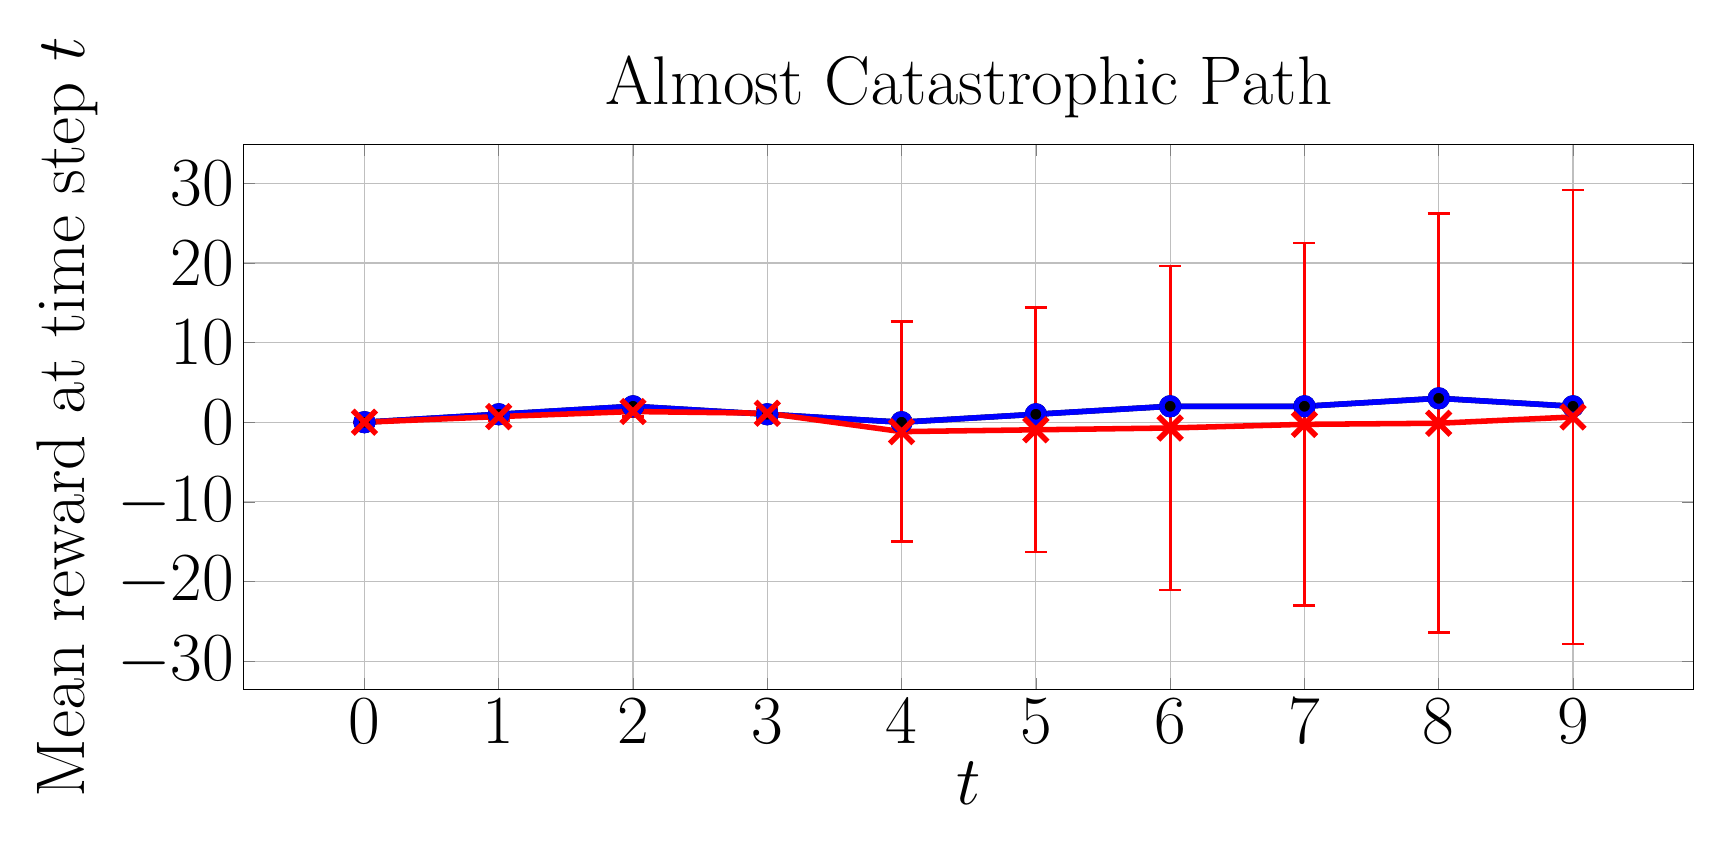
\begin{tikzpicture}
                \begin{axis}[
                    xlabel={$t$},
                    ylabel={Mean reward at time step $t$},
                    title={Almost Catastrophic Path},
                    grid=both,
                    width=20cm, height=8.5cm,
                    every axis/.style={font=\Huge},
                    %
                ]
                \addplot[
                    color=black, %
                    mark=*, %
                    line width=2pt,
                    mark size=3pt,
                    error bars/.cd,
                    y dir=both, %
                    y explicit, %
                    error bar style={line width=1pt,solid},
                    error mark options={line width=1pt,mark size=4pt,rotate=90}
                ]
                coordinates {
                    (0, 0.0)  +- (0, 0.0)
                    (1, 1.0)  +- (0, 0.0) 
                    (2, 2.0)  +- (0, 0.0) 
                    (3, 1.0)  +- (0, 0.0)
                    (4, 0.0)  +- (0, 0.0)
                    (5, 1.0) +- (0, 0.0)
                    (6, 2.0) +- (0, 0.0)
                    (7, 2.0) +- (0, 0.0)
                    (8, 3.0) +- (0, 0.0)
                    (9, 2.0) +- (0, 0.0)
                };
                %
                \addplot[
                    color=blue, %
                    mark=o, %
                    line width=2pt,
                    mark size=3pt,
                    error bars/.cd,
                    y dir=both, %
                    y explicit, %
                    error bar style={line width=1pt,solid},
                    error mark options={line width=1pt,mark size=4pt,rotate=90}
                ]
                coordinates {
                    (0, 0.0)  +- (0, 0.0)
                    (1, 1.0)  +- (0, 0.0) 
                    (2, 2.0)  +- (0, 0.0) 
                    (3, 1.0)  +- (0, 0.0)
                    (4, 0.0)  +- (0, 0.0)
                    (5, 1.0) +- (0, 0.0)
                    (6, 2.0) +- (0, 0.0)
                    (7, 2.0) +- (0, 0.0)
                    (8, 3.0) +- (0, 0.0)
                    (9, 2.0) +- (0, 0.0)
                };
                %
                \addplot[
                    color=red, %
                    mark=x, %
                    line width=2pt,
                    mark size=6pt,
                    error bars/.cd,
                    y dir=both, %
                    y explicit, %
                    error bar style={line width=1pt,solid},
                    error mark options={line width=1pt,mark size=4pt,rotate=90}
                ]
                coordinates {
                    (0, 0.0)  +- (0, 0.0)
                    (1, 0.7065655)  +- (0, 0.4553358) 
                    (2, 1.341673)  +- (0, 0.67091621) 
                    (3, 1.122926)  +- (0, 0.61281824)
                    (4, -1.1821935)  +- (0, 13.82444042)
                    (5, -0.952399)  +- (0, 15.35195457)
                    (6, -0.72672) +- (0, 20.33508414)
                    (7, -0.268983) +- (0, 22.77861454)
                    (8, -0.1310835) +- (0, 26.31013314)
                    (9, 0.65806) +- (0, 28.50670214)
                };
                %
            %
            %
            %
            %
            %
            %
            %
            %
            %
            %
            %
            %
            %
            %
            %
            %
            %
            %
                \end{axis}
            \end{tikzpicture}
         }
    }
    \hspace{1cm}
    \subfigure[\footnotesize Lowest cumulative reward: Interval CFMDP ($-698$), Gumbel-max SCM ($-698$)]{%
         \resizebox{0.76\columnwidth}{!}{
            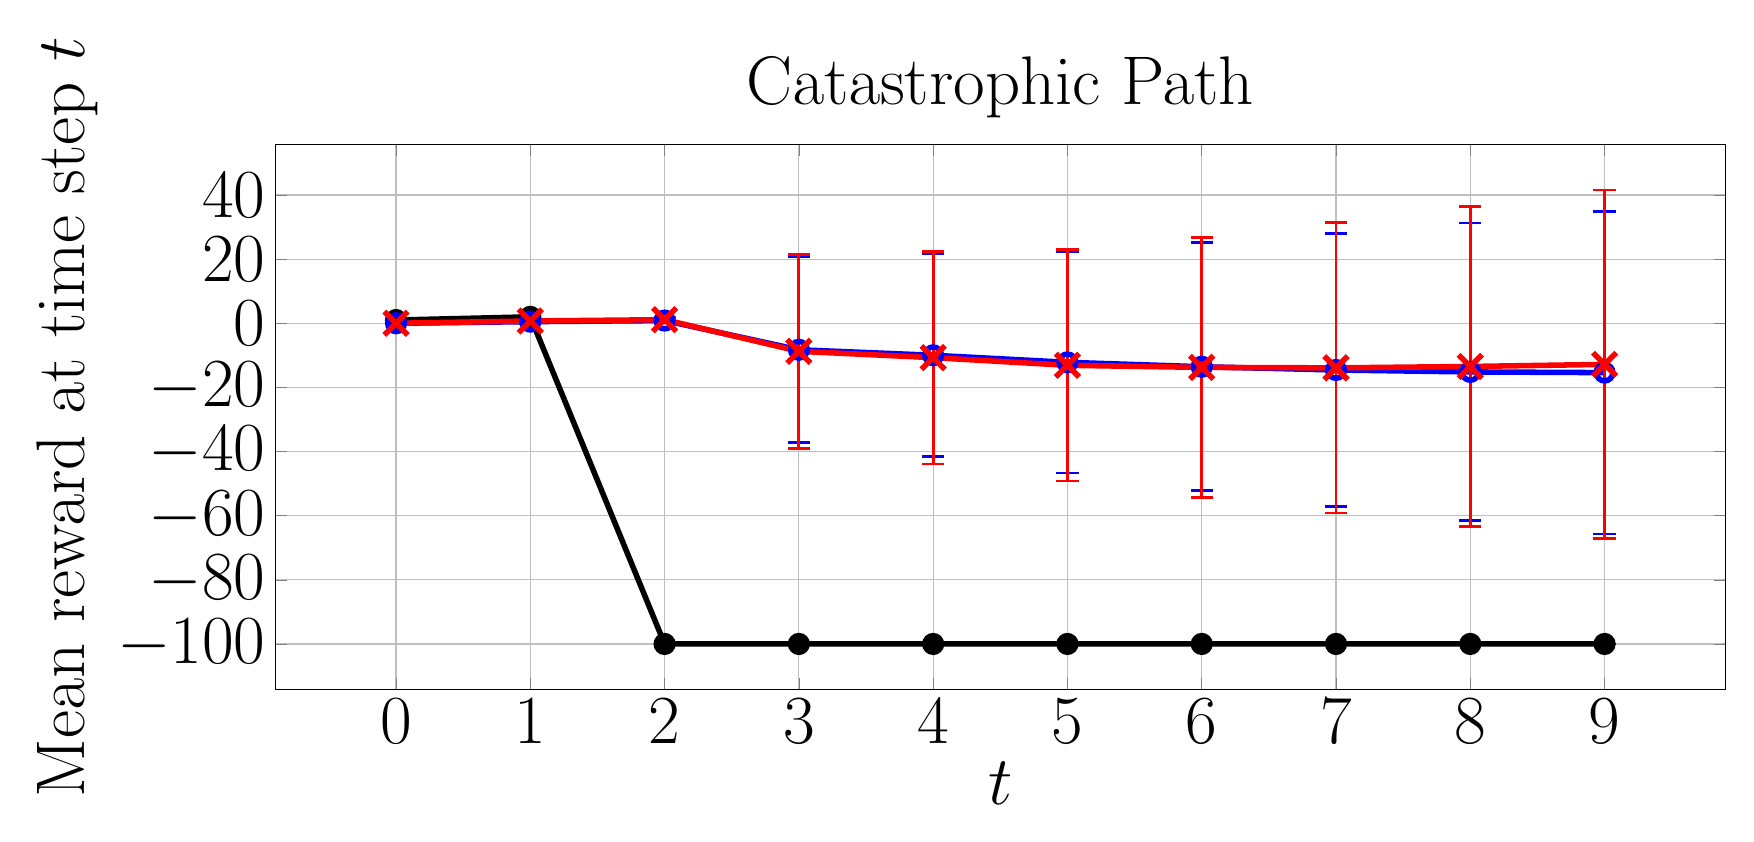
\begin{tikzpicture}
                \begin{axis}[
                    xlabel={$t$},
                    ylabel={Mean reward at time step $t$},
                    title={Catastrophic Path},
                    grid=both,
                    width=20cm, height=8.5cm,
                    every axis/.style={font=\Huge},
                    %
                ]
                \addplot[
                    color=black, %
                    mark=*, %
                    line width=2pt,
                    mark size=3pt,
                    error bars/.cd,
                    y dir=both, %
                    y explicit, %
                    error bar style={line width=1pt,solid},
                    error mark options={line width=1pt,mark size=4pt,rotate=90}
                ]
                coordinates {
                    (0, 1.0)  +- (0, 0.0)
                    (1, 2.0)  +- (0, 0.0) 
                    (2, -100.0)  +- (0, 0.0) 
                    (3, -100.0)  +- (0, 0.0)
                    (4, -100.0)  +- (0, 0.0)
                    (5, -100.0) +- (0, 0.0)
                    (6, -100.0) +- (0, 0.0)
                    (7, -100.0) +- (0, 0.0)
                    (8, -100.0) +- (0, 0.0)
                    (9, -100.0) +- (0, 0.0)
                };
                %
                \addplot[
                    color=blue, %
                    mark=o, %
                    line width=2pt,
                    mark size=3pt,
                    error bars/.cd,
                    y dir=both, %
                    y explicit, %
                    error bar style={line width=1pt,solid},
                    error mark options={line width=1pt,mark size=4pt,rotate=90}
                ]
                coordinates {
                    (0, 0.0)  +- (0, 0.0)
                    (1, 0.504814)  +- (0, 0.49997682) 
                    (2, 0.8439835)  +- (0, 0.76831917) 
                    (3, -8.2709165)  +- (0, 28.93656754)
                    (4, -9.981082)  +- (0, 31.66825363)
                    (5, -12.1776325) +- (0, 34.53463233)
                    (6, -13.556076) +- (0, 38.62845372)
                    (7, -14.574418) +- (0, 42.49603359)
                    (8, -15.1757075) +- (0, 46.41913968)
                    (9, -15.3900395) +- (0, 50.33563368)
                };
                %
                \addplot[
                    color=red, %
                    mark=x, %
                    line width=2pt,
                    mark size=6pt,
                    error bars/.cd,
                    y dir=both, %
                    y explicit, %
                    error bar style={line width=1pt,solid},
                    error mark options={line width=1pt,mark size=4pt,rotate=90}
                ]
                coordinates {
                    (0, 0.0)  +- (0, 0.0)
                    (1, 0.701873)  +- (0, 0.45743556) 
                    (2, 1.1227805)  +- (0, 0.73433129) 
                    (3, -8.7503255)  +- (0, 30.30257976)
                    (4, -10.722092)  +- (0, 33.17618589)
                    (5, -13.10721)  +- (0, 36.0648089)
                    (6, -13.7631645) +- (0, 40.56553451)
                    (7, -13.909043) +- (0, 45.23829402)
                    (8, -13.472517) +- (0, 49.96270296)
                    (9, -12.8278835) +- (0, 54.38618735)
                };
                %
            %
            %
            %
            %
            %
            %
            %
            %
            %
            %
            %
            %
            %
            %
            %
            %
            %
            %
                \end{axis}
            \end{tikzpicture}
         }
    }
    \caption{Average instant reward of CF paths induced by policies on GridWorld $p=0.4$.}
    \label{fig: reward p=0.4}
\end{figure*}

\subsection{Experimental Setup}
To compare policy performance, we measure the average rewards of counterfactual paths induced by our policy and the Gumbel-max policy by uniformly sampling $200$ counterfactual MDPs from the ICFMDP and generating $10,000$ counterfactual paths over each sampled CFMDP. \jl{Since the interval CFMDP depends on the observed path, we select $4$  paths of varying optimality to evaluate how the observed path impacts the performance of both policies: an optimal path, a slightly suboptimal path that could reach the optimal reward with a few changes, a catastrophic path that enters a catastrophic, terminal state with low reward, and an almost catastrophic path that was close to entering a catastrophic state.} When measuring the average probability bound widths and execution time needed to generate the ICFMDPs, we averaged over $20$ randomly generated observed paths
\footnote{Further training details are provided in Appendix \ref{app: training details}, and the code is provided at \href{https://github.com/ddv-lab/robust-cf-inference-in-MDPs}{https://github.com/ddv-lab/robust-cf-inference-in-MDPs}
%
%
.}.

\subsection{GridWorld}
\jl{The GridWorld MDP is a $4 \times 4$ grid where an agent must navigate from the top-left corner to the goal state in the bottom-right corner, avoiding a dangerous terminal state in the centre. At each time step, the agent can move up, down, left, or right, but there is a small probability (controlled by hyper-parameter $p$) of moving in an unintended direction. As the agent nears the goal, the reward for each state increases, culminating in a reward of $+100$ for reaching the goal. Entering the dangerous state results in a penalty of $-100$. We use two versions of GridWorld: a less stochastic version with $p=0.9$ (i.e., $90$\% chance of moving in the chosen direction) and a more stochastic version with $p=0.4$.}

\paragraph{GridWorld ($p=0.9$)}
When $p=0.9$, the counterfactual probability bounds are typically narrow (see Table \ref{tab:nonzero_probs} for average measurements). Consequently, as shown in Figure \ref{fig: reward p=0.9}, both policies are nearly identical and perform similarly well across the optimal, slightly suboptimal, and catastrophic paths.
%
However, for the almost catastrophic path, the interval CFMDP path is more conservative and follows the observed path more closely (as this is where the probability bounds are narrowest), which typically requires one additional step to reach the goal state than the Gumbel-max SCM policy.
%

\paragraph{GridWorld ($p=0.4$)}
\jl{When $p=0.4$, the GridWorld environment becomes more uncertain, increasing the risk of entering the dangerous state even if correct actions are chosen. Thus, as shown in Figure \ref{fig: reward p=0.4}, the interval CFMDP policy adopts a more conservative approach, avoiding deviation from the observed policy if it cannot guarantee higher counterfactual rewards (see the slightly suboptimal and almost catastrophic paths), whereas the Gumbel-max SCM is inconsistent: it can yield higher rewards, but also much lower rewards, reflected in the wide error bars.} For the catastrophic path, both policies must deviate from the observed path to achieve a higher reward and, in this case, perform similarly.
%
%
%
%
\subsection{Sepsis}
The Sepsis MDP \citep{oberst2019counterfactual} simulates trajectories of Sepsis patients. Each state consists of four vital signs (heart rate, blood pressure, oxygen concentration, and glucose levels), categorised as low, normal, or high.
and three treatments that can be toggled on/off at each time step (8 actions in total). Unlike \citet{oberst2019counterfactual}, we scale rewards based on the number of out-of-range vital signs, between $-1000$ (patient dies) and $1000$ (patient discharged). \jl{Like the GridWorld $p=0.4$ experiment, the Sepsis MDP is highly uncertain, as many states are equally likely to lead to optimal and poor outcomes. Thus, as shown in Figure \ref{fig: reward sepsis}, both policies follow the observed optimal and almost catastrophic paths to guarantee rewards are no worse than the observation.} However, improving the catastrophic path requires deviating from the observation. Here, the Gumbel-max SCM policy, on average, performs better than the interval CFMDP policy. But, since both policies have lower bounds clipped at $-1000$, neither policy reliably improves over the observation. In contrast, for the slightly suboptimal path, the interval CFMDP policy performs significantly better, shown by its higher lower bounds. 
Moreover, in these two cases, the worst-case counterfactual path generated by the interval CFMDP policy is better than that of the Gumbel-max SCM policy,
indicating its greater robustness.
%
\begin{figure*}
    \centering
     \resizebox{0.6\textwidth}{!}{
        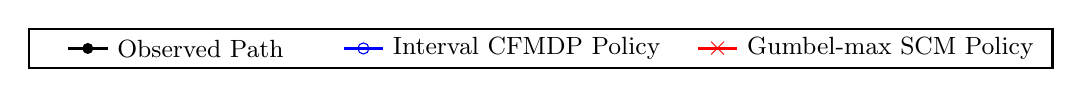
\begin{tikzpicture}[scale=1.0, every node/.style={scale=1.0}]
            \draw[thick, black] (-3, -0.25) rectangle (10, 0.25);
            %
            \draw[black, line width=1pt] (-2.5, 0.0) -- (-2,0.0);
            \fill[black] (-2.25,0.0) circle (2pt); %
            \node[right] at (-2,0.0) {\small Observed Path};
            
            %
            \draw[blue, line width=1pt] (1.0,0.0) -- (1.5,0.0);
            \node[draw=blue, circle, minimum size=4pt, inner sep=0pt] at (1.25,0.0) {}; %
            \node[right] at (1.5,0.0) {\small Interval CFMDP Policy};
            
            %
            \draw[red, line width=1pt] (5.5,0) -- (6,0);
            \node[red] at (5.75,0) {$\boldsymbol{\times}$}; %
            \node[right] at (6,0) {\small Gumbel-max SCM Policy};
        \end{tikzpicture}
    }\\
    \subfigure[\footnotesize Lowest cumulative reward: Interval CFMDP ($8000$), Gumbel-max SCM ($8000$)]{%
         \resizebox{0.76\columnwidth}{!}{
             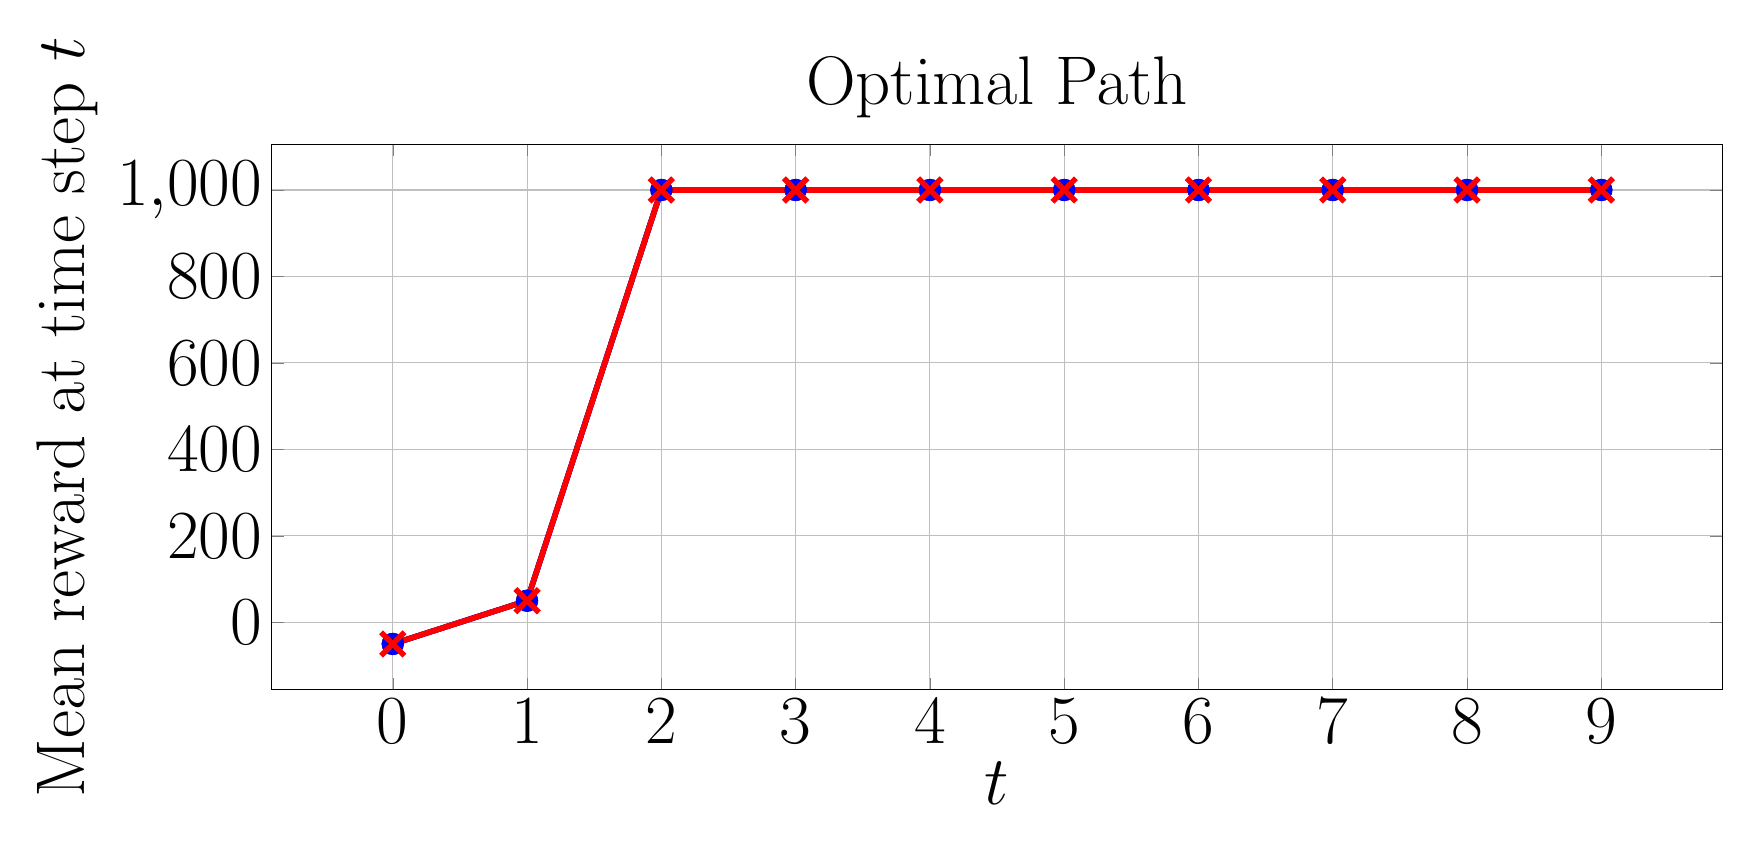
\begin{tikzpicture}
                \begin{axis}[
                    xlabel={$t$},
                    ylabel={Mean reward at time step $t$},
                    title={Optimal Path},
                    grid=both,
                    width=20cm, height=8.5cm,
                    every axis/.style={font=\Huge},
                    %
                ]
                \addplot[
                    color=black, %
                    mark=*, %
                    line width=2pt,
                    mark size=3pt,
                ]
                coordinates {
                    (0, -50.0)
                    (1, 50.0)
                    (2, 1000.0)
                    (3, 1000.0)
                    (4, 1000.0)
                    (5, 1000.0)
                    (6, 1000.0)
                    (7, 1000.0)
                    (8, 1000.0)
                    (9, 1000.0)
                };
                %
                \addplot[
                    color=blue, %
                    mark=o, %
                    line width=2pt,
                    mark size=3pt,
                    error bars/.cd,
                    y dir=both, %
                    y explicit, %
                    error bar style={line width=1pt,solid},
                    error mark options={line width=1pt,mark size=4pt,rotate=90}
                ]
                coordinates {
                    (0, -50.0)  +- (0, 0.0)
                    (1, 50.0)  +- (0, 0.0) 
                    (2, 1000.0)  +- (0, 0.0) 
                    (3, 1000.0)  +- (0, 0.0)
                    (4, 1000.0)  +- (0, 0.0)
                    (5, 1000.0) +- (0, 0.0)
                    (6, 1000.0) +- (0, 0.0)
                    (7, 1000.0) +- (0, 0.0)
                    (8, 1000.0) +- (0, 0.0)
                    (9, 1000.0) +- (0, 0.0)
                };
                %
                \addplot[
                    color=red, %
                    mark=x, %
                    line width=2pt,
                    mark size=6pt,
                    error bars/.cd,
                    y dir=both, %
                    y explicit, %
                    error bar style={line width=1pt,solid},
                    error mark options={line width=1pt,mark size=4pt,rotate=90}
                ]
                coordinates {
                    (0, -50.0)  +- (0, 0.0)
                    (1, 50.0)  +- (0, 0.0) 
                    (2, 1000.0)  +- (0, 0.0) 
                    (3, 1000.0)  +- (0, 0.0)
                    (4, 1000.0)  +- (0, 0.0)
                    (5, 1000.0) +- (0, 0.0)
                    (6, 1000.0) +- (0, 0.0)
                    (7, 1000.0) +- (0, 0.0)
                    (8, 1000.0) +- (0, 0.0)
                    (9, 1000.0) +- (0, 0.0)
                };
                %
                \end{axis}
            \end{tikzpicture}
         }
    }
    \hspace{1cm}
    \subfigure[\footnotesize Lowest cumulative reward: Interval CFMDP ($-5980$), Gumbel-max SCM ($-8000$)]{%
         \resizebox{0.76\columnwidth}{!}{
            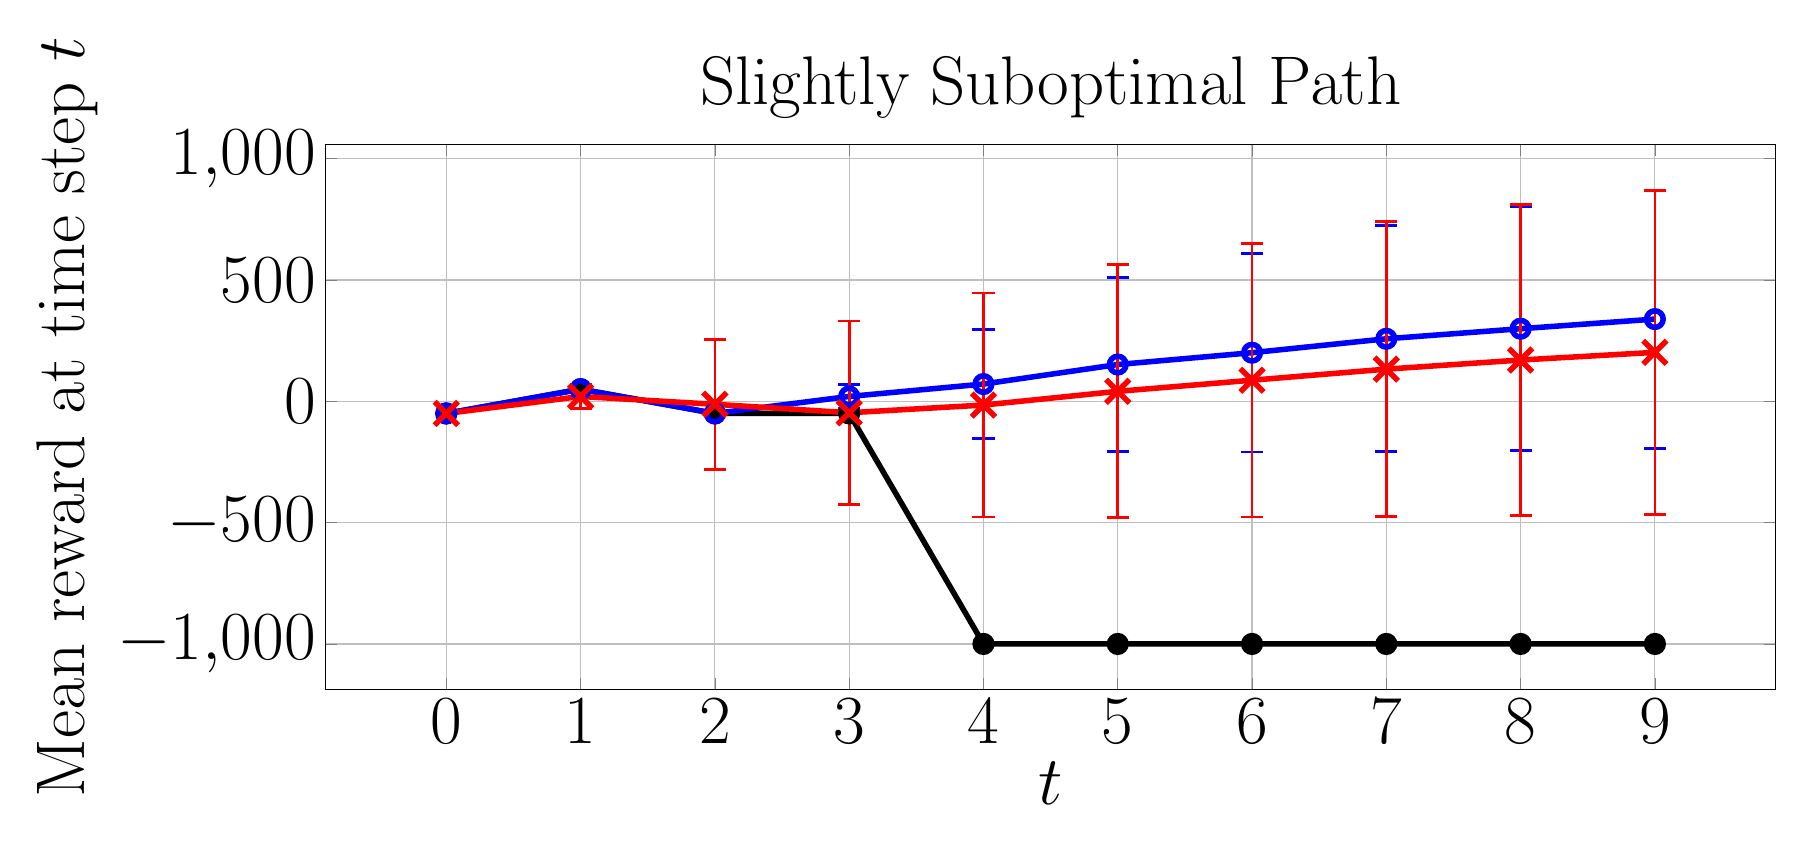
\begin{tikzpicture}
                \begin{axis}[
                    xlabel={$t$},
                    ylabel={Mean reward at time step $t$},
                    title={Slightly Suboptimal Path},
                    grid=both,
                    width=20cm, height=8.5cm,
                    every axis/.style={font=\Huge},
                    %
                ]
               \addplot[
                    color=black, %
                    mark=*, %
                    line width=2pt,
                    mark size=3pt,
                ]
                coordinates {
                    (0, -50.0)
                    (1, 50.0)
                    (2, -50.0)
                    (3, -50.0)
                    (4, -1000.0)
                    (5, -1000.0)
                    (6, -1000.0)
                    (7, -1000.0)
                    (8, -1000.0)
                    (9, -1000.0)
                };
                %
                \addplot[
                    color=blue, %
                    mark=o, %
                    line width=2pt,
                    mark size=3pt,
                    error bars/.cd,
                    y dir=both, %
                    y explicit, %
                    error bar style={line width=1pt,solid},
                    error mark options={line width=1pt,mark size=4pt,rotate=90}
                ]
                coordinates {
                    (0, -50.0)  +- (0, 0.0)
                    (1, 50.0)  +- (0, 0.0) 
                    (2, -50.0)  +- (0, 0.0) 
                    (3, 20.0631)  +- (0, 49.97539413)
                    (4, 71.206585)  +- (0, 226.02033693)
                    (5, 151.60797) +- (0, 359.23292559)
                    (6, 200.40593) +- (0, 408.86185176)
                    (7, 257.77948) +- (0, 466.10372804)
                    (8, 299.237465) +- (0, 501.82579506)
                    (9, 338.9129) +- (0, 532.06124996)
                };
                %
                \addplot[
                    color=red, %
                    mark=x, %
                    line width=2pt,
                    mark size=6pt,
                    error bars/.cd,
                    y dir=both, %
                    y explicit, %
                    error bar style={line width=1pt,solid},
                    error mark options={line width=1pt,mark size=4pt,rotate=90}
                ]
                coordinates {
                    (0, -50.0)  +- (0, 0.0)
                    (1, 20.00736)  +- (0, 49.99786741) 
                    (2, -12.282865)  +- (0, 267.598755) 
                    (3, -47.125995)  +- (0, 378.41755832)
                    (4, -15.381965)  +- (0, 461.77616558)
                    (5, 41.15459) +- (0, 521.53189262)
                    (6, 87.01595) +- (0, 564.22243126 )
                    (7, 132.62376) +- (0, 607.31338037)
                    (8, 170.168145) +- (0, 641.48013693)
                    (9, 201.813135) +- (0, 667.29441777)
                };
                %
                %
                %
                %
                %
                %
                %
                %
                %
                %
                %
                %
                %
                %
                %
                %
                %
                %
                %
                \end{axis}
            \end{tikzpicture}
         }
    }\\[-1.5pt]
    \subfigure[\footnotesize Lowest cumulative reward: Interval CFMDP ($100$), Gumbel-max SCM ($100$)]{%
         \resizebox{0.76\columnwidth}{!}{
             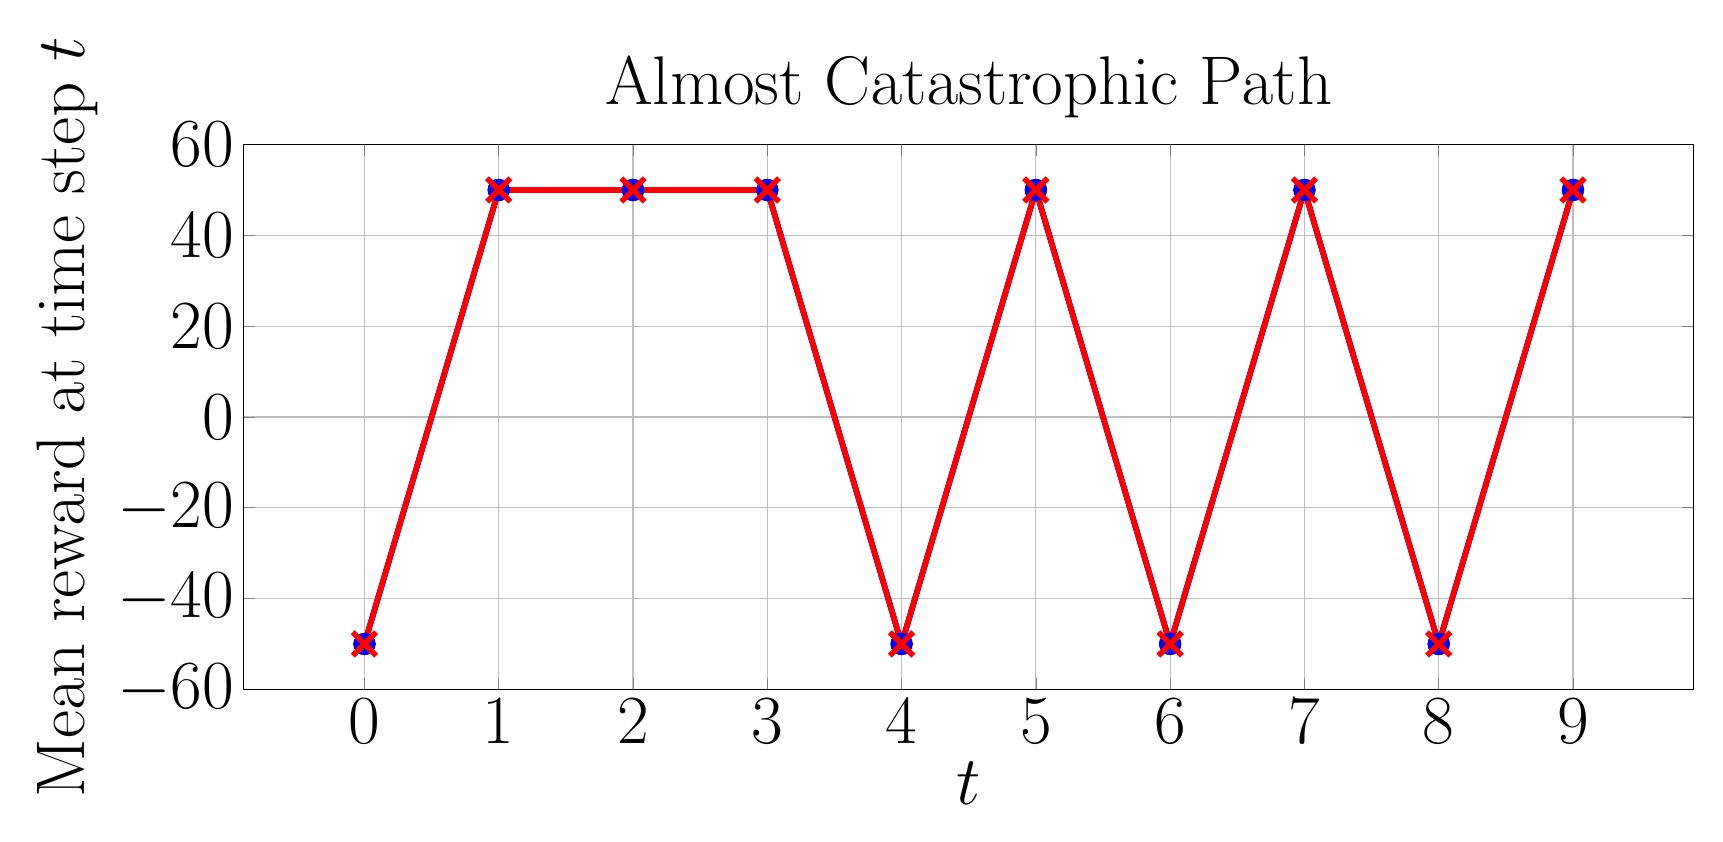
\begin{tikzpicture}
                \begin{axis}[
                    xlabel={$t$},
                    ylabel={Mean reward at time step $t$},
                    title={Almost Catastrophic Path},
                    grid=both,
                    every axis/.style={font=\Huge},
                    width=20cm, height=8.5cm,
                    %
                ]
               \addplot[
                    color=black, %
                    mark=*, %
                    line width=2pt,
                    mark size=3pt,
                ]
                coordinates {
                    (0, -50.0)
                    (1, 50.0)
                    (2, 50.0)
                    (3, 50.0)
                    (4, -50.0)
                    (5, 50.0)
                    (6, -50.0)
                    (7, 50.0)
                    (8, -50.0)
                    (9, 50.0)
                };
                %
                %
                \addplot[
                    color=blue, %
                    mark=o, %
                    line width=2pt,
                    mark size=3pt,
                    error bars/.cd,
                    y dir=both, %
                    y explicit, %
                    error bar style={line width=1pt,solid},
                    error mark options={line width=1pt,mark size=4pt,rotate=90}
                ]
                coordinates {
                    (0, -50.0)  +- (0, 0.0)
                    (1, 50.0)  +- (0, 0.0) 
                    (2, 50.0)  +- (0, 0.0) 
                    (3, 50.0)  +- (0, 0.0)
                    (4, -50.0)  +- (0, 0.0)
                    (5, 50.0) +- (0, 0.0)
                    (6, -50.0) +- (0, 0.0)
                    (7, 50.0) +- (0, 0.0)
                    (8, -50.0) +- (0, 0.0)
                    (9, 50.0) +- (0, 0.0)
                };
                %
                \addplot[
                    color=red, %
                    mark=x, %
                    line width=2pt,
                    mark size=6pt,
                    error bars/.cd,
                    y dir=both, %
                    y explicit, %
                    error bar style={line width=1pt,solid},
                    error mark options={line width=1pt,mark size=4pt,rotate=90}
                ]
                coordinates {
                    (0, -50.0)  +- (0, 0.0)
                    (1, 50.0)  +- (0, 0.0) 
                    (2, 50.0)  +- (0, 0.0) 
                    (3, 50.0)  +- (0, 0.0)
                    (4, -50.0)  +- (0, 0.0)
                    (5, 50.0) +- (0, 0.0)
                    (6, -50.0) +- (0, 0.0)
                    (7, 50.0) +- (0, 0.0)
                    (8, -50.0) +- (0, 0.0)
                    (9, 50.0) +- (0, 0.0)
                };
                %
                %
                %
                %
                %
                %
                %
                %
                %
                %
                %
                %
                %
                %
                %
                %
                %
                %
                %
                \end{axis}
            \end{tikzpicture}
         }
    }
    \hspace{1cm}
    \subfigure[\footnotesize Lowest cumulative reward: Interval CFMDP ($-7150$), Gumbel-max SCM ($-9050$)]{%
         \resizebox{0.76\columnwidth}{!}{
            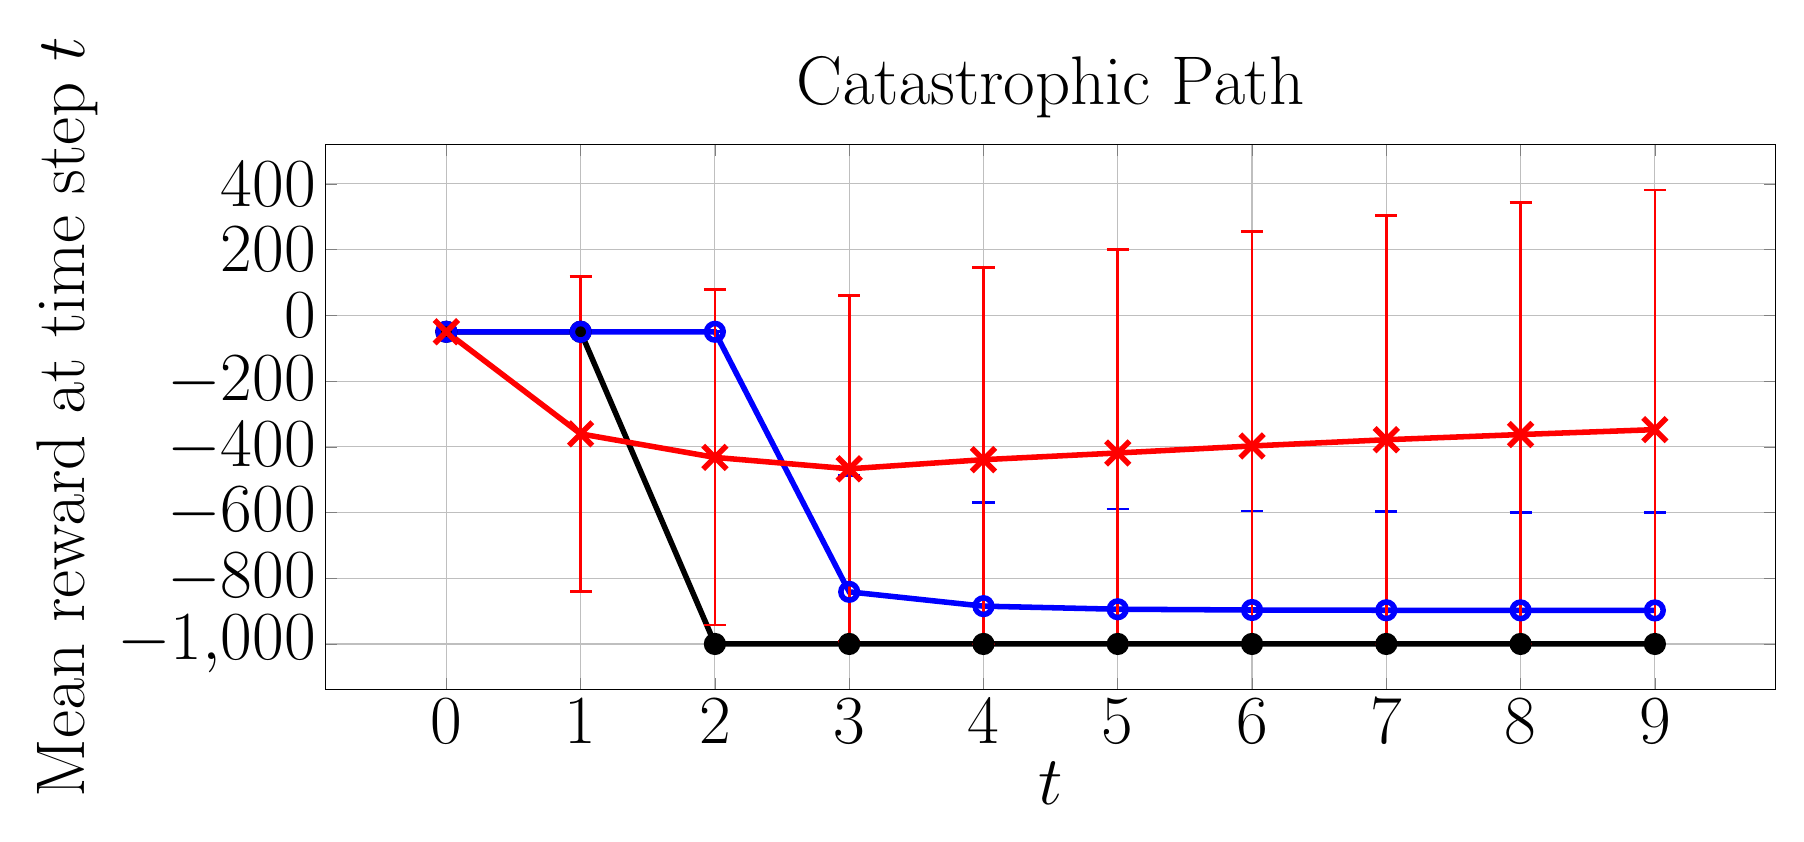
\begin{tikzpicture}
                \begin{axis}[
                    xlabel={$t$},
                    ylabel={Mean reward at time step $t$},
                    title={Catastrophic Path},
                    grid=both,
                    width=20cm, height=8.5cm,
                    every axis/.style={font=\Huge},
                    %
                ]
               \addplot[
                    color=black, %
                    mark=*, %
                    line width=2pt,
                    mark size=3pt,
                ]
                coordinates {
                    (0, -50.0)
                    (1, -50.0)
                    (2, -1000.0)
                    (3, -1000.0)
                    (4, -1000.0)
                    (5, -1000.0)
                    (6, -1000.0)
                    (7, -1000.0)
                    (8, -1000.0)
                    (9, -1000.0)
                };
                %
                %
                \addplot[
                    color=blue, %
                    mark=o, %
                    line width=2pt,
                    mark size=3pt,
                    error bars/.cd,
                    y dir=both, %
                    y explicit, %
                    error bar style={line width=1pt,solid},
                    error mark options={line width=1pt,mark size=4pt,rotate=90}
                ]
                coordinates {
                    (0, -50.0)  +- (0, 0.0)
                    (1, -50.0)  +- (0, 0.0) 
                    (2, -50.0)  +- (0, 0.0) 
                    (3, -841.440725)  += (0, 354.24605512) -= (0, 158.559275)
                    (4, -884.98225)  += (0, 315.37519669) -= (0, 115.01775)
                    (5, -894.330425) += (0, 304.88572805) -= (0, 105.669575)
                    (6, -896.696175) += (0, 301.19954514) -= (0, 103.303825)
                    (7, -897.4635) += (0, 299.61791279) -= (0, 102.5365)
                    (8, -897.77595) += (0, 298.80392585) -= (0, 102.22405)
                    (9, -897.942975) += (0, 298.32920557) -= (0, 102.057025)
                };
                %
                \addplot[
                    color=red, %
                    mark=x, %
                    line width=2pt,
                    mark size=6pt,
                    error bars/.cd,
                    y dir=both, %
                    y explicit, %
                    error bar style={line width=1pt,solid},
                    error mark options={line width=1pt,mark size=4pt,rotate=90}
                ]
            coordinates {
                    (0, -50.0)  +- (0, 0.0)
                    (1, -360.675265)  +- (0, 479.39812699) 
                    (2, -432.27629)  +- (0, 510.38620897) 
                    (3, -467.029545)  += (0, 526.36009628) -= (0, 526.36009628)
                    (4, -439.17429)  += (0, 583.96638919) -= (0, 560.82571)
                    (5, -418.82704) += (0, 618.43027478) -= (0, 581.17296)
                    (6, -397.464895) += (0, 652.67322574) -= (0, 602.535105)
                    (7, -378.49052) += (0, 682.85407033) -= (0, 621.50948)
                    (8, -362.654195) += (0, 707.01412023) -= (0, 637.345805)
                    (9, -347.737935) += (0, 729.29076479) -= (0, 652.262065)
                };
                %
                %
                %
                %
                %
                %
                %
                %
                %
                %
                %
                %
                %
                %
                %
                %
                %
                %
                %
                \end{axis}
            \end{tikzpicture}
         }
    }
    \caption{Average instant reward of CF paths induced by policies on Sepsis.}
    \label{fig: reward sepsis}
\end{figure*}

%
%
%
\subsection{Interval CFMDP Bounds}
%
%
Table \ref{tab:nonzero_probs} presents the mean counterfactual probability bound widths (excluding transitions where the upper bound is $0$) for each MDP, averaged over 20 observed paths. We compare the bounds under counterfactual stability (CS) and monotonicity (M) assumptions, CS alone, and no assumptions. This shows that the assumptions marginally reduce the bound widths, indicating the assumptions tighten the bounds without excluding too many causal models, as intended.
\renewcommand{\arraystretch}{1}

\begin{table}
\centering
\caption{Mean width of counterfactual probability bounds}
\resizebox{0.8\columnwidth}{!}{%
\begin{tabular}{|c|c|c|c|}
\hline
\multirow{2}{*}{\textbf{Environment}} & \multicolumn{3}{c|}{\textbf{Assumptions}} \\ \cline{2-4}
 & \textbf{CS + M} & \textbf{CS} & \textbf{None\tablefootnote{\jl{Equivalent to \citet{li2024probabilities}'s bounds (see Section \ref{sec: equivalence with Li}).}}} \\ \hline
\textbf{GridWorld} ($p=0.9$) & 0.0817 & 0.0977 & 0.100 \\ \hline
\textbf{GridWorld} ($p=0.4$) & 0.552  & 0.638  & 0.646 \\ \hline
\textbf{Sepsis} & 0.138 & 0.140 & 0.140 \\ \hline
\end{tabular}
}
\label{tab:nonzero_probs}
\end{table}


\subsection{Execution Times}
Table \ref{tab: times} compares the average time needed to generate the interval CFMDP vs.\ the Gumbel-max SCM CFMDP for 20 observations.
The GridWorld algorithms were run single-threaded, while the Sepsis experiments were run in parallel.
Generating the interval CFMDP is significantly faster as it uses exact analytical bounds, whereas the Gumbel-max CFMDP requires sampling from the Gumbel distribution to estimate counterfactual transition probabilities. \jl{Since constructing the counterfactual MDP models is the main bottleneck in both approaches, ours is more efficient overall and suitable for larger MDPs.}
\begin{table}
\centering
\caption{Mean execution time to generate CFMDPs}
\resizebox{0.99\columnwidth}{!}{%
\begin{tabular}{|c|c|c|}
\hline
\multirow{2}{*}{\textbf{Environment}} & \multicolumn{2}{c|}{\textbf{Mean Execution Time (s)}} \\ \cline{2-3} 
                                      & \textbf{Interval CFMDP} & \textbf{Gumbel-max CFMDP} \\ \hline
\textbf{GridWorld ($p=0.9$) }                  & 0.261                   & 56.1                      \\ \hline
\textbf{GridWorld ($p=0.4$)  }                 & 0.336                   & 54.5                      \\ \hline
\textbf{Sepsis}                                 & 688                     & 2940                      \\ \hline
\end{tabular}%
}
\label{tab: times}
\end{table}

\section{Results}
\label{sec:Results}

In this section, we present various analysis results that demonstrate the adoption of code obfuscation in Google Play.

\subsection{Overall Obfuscation Trends} 
\label{sec:obstrend}

\subsubsection{Presence of obfuscation} Out of the 548,967 Google Play Store APKs analyzed, we identified 308,782 obfuscated apps, representing approximately 56.25\% of the total. In Figure~\ref{fig:obfuscated_percentage}, we show the year-wise percentage of obfuscated apps for 2016-2023. There is an overall obfuscation increase of 13\% between 2016 and 2023, and as can be seen, the percentage of obfuscated apps has been increasing in the last few years, barring 2019 and 2020. As explained in Section~\ref{subsec:dataset}, 2019 and 2020 contain apps that are more likely to be abandoned by developers, and as such, they may not use advanced development practices.

\begin{figure}[h!]
\centering
    \includegraphics[width=\linewidth]{Figures/Only_obfuscation_trendV2.pdf}
    \caption{Percentage of obfuscated apps by year} \vspace{-4mm}
    \label{fig:obfuscated_percentage}
\end{figure}


From 2016 to 2018, the obfuscation levels were relatively stable at around 50-55\%, while from 2021 to 2023, there was a marked rise, reaching approximately 66\% in 2023. This indicates a growing focus on app protection measures among developers, likely driven by heightened security and IP concerns and the availability of advanced obfuscation tools.


\subsubsection{Obfuscation tools} Among the obfuscated APKs, our tool detector identified that 40.92\% of the apps use Proguard, 36.64\% use Allatori, 1.01\% use DashO, and 21.43\% use other (i.e., unknown) tools. We show the yearly trends in Figure~\ref{fig:ofbuscated_tool}. Note that we omit results in 2019 and 2020 ({\bf cf.} Section~\ref{subsec:dataset}).

ProGuard and Allatori are the most consistently used obfuscation tools, with ProGuard showing a slight overall increase in popularity and Allatori demonstrating variability. This inclination could be attributed to ProGuard being the default obfuscator integrated into Android Studio, a widely used development environment for Android applications. Notably, ProGuard usage increased by 13\% from 2018 to 2021, likely due to the introduction of R8 in April 2019~\cite{release_note_android}, which further simplified ProGuard integration with Android apps.

\begin{figure}[h]
\centering
    \includegraphics[width=\linewidth]{Figures/Initial_Tool_Trend_2019_dropV2.pdf} 
    \caption{Yearly obfuscation tool usage}
    \label{fig:ofbuscated_tool}
\end{figure}


DashO consistently remains low in usage, likely due to its high cost. The use of other obfuscation tools decreased until 2018 but has shown a resurgence from 2021 to 2023. This suggests that developers might be using other or custom tools, or our detector might be predicting some apps obfuscated with Proguard or Allatori as `other.' To investigate, we manually checked a sample of apps from the `other' category and confirmed they are indeed obfuscated. However, we could not determine which obfuscation tools the developers used. We discuss this potential limitation further in Section~\ref{sec:limitations}.


\subsubsection{Obfuscation techniques} We show the year-wise breakdown of obfuscation technique usage in Figure~\ref{fig:obfuscated_tech}. Among the various obfuscation techniques, Identifier Renaming emerged as the most prevalent, with 99.62\% of obfuscated apps using it alone or in combination with other methods (Categories of Only IR, IR and CF, IR and SE, or All three). Furthermore, 81.04\% of obfuscated apps used Control Flow Modification, and 62.76\% used String Encryption. The pervasive use of Identifier Renaming (IR) can be attributed to the fact that all obfuscation tools support it ({\bf cf.} Table~\ref{tab:ob_tool_cap}). Similarly, lower adoption of Control Flow Modification and String Encryption can be attributed to Proguard not supporting it. 

\begin{figure}[h]
\centering
    \includegraphics[width=\linewidth]{Figures/Initial_Tech_Trend_2019_dropV2.pdf} 
    \caption{Yearly obfuscation technique usage}
    \label{fig:obfuscated_tech}
\end{figure}



Next, we investigate the adoption of obfuscation on Google Play Store from various perspectives. Same as earlier, due to the smaller dataset size and possible bias ({\bf cf.} Section~\ref{subsec:dataset}), we exclude the APKs from 2019 and 2020 from this analyses.


\subsection{App Genre}
\label{sec:app_genre}

First, we investigate whether the obfuscation practices vary according to the App genre. Initially, we analysed all the APKs together before separating them into two snapshots.


\begin{figure*}[h]
    \centering
    \includegraphics[width=\linewidth]{Figures/AppGenreObfuscationV3.pdf}
    \caption{Obfuscated app percentage by genre (overall)}
    \label{fig:app_genre_overall}
\end{figure*}

Figure~\ref{fig:app_genre_overall} shows the genre-wise obfuscated app percentage. We note that 19 genres have more than 60\% of the apps obfuscated, and almost all the genres have more than 40\% obfuscation percentage. \textit{Casino} genre has the highest obfuscation percentage rate at 80\%, and overall, game genres tend to be more obfuscated than the other genres. The higher obfuscation usage in casino apps is logical due to their nature. These apps often simulate or involve gambling activities and handle monetary transactions and sensitive data related to in-game purchases, making them attractive targets for reverse engineering and hacking. This necessitates robust security measures to prevent fraud and protect user data. 


\begin{figure}[h]
    \centering
    \includegraphics[width=\linewidth]{Figures/AppGenre2018_2023ComparisonV3.pdf}
    \caption{Percentage of obfuscated apps by genre (2018-2023)}
    \label{fig:app_genre_comparison}
\end{figure}



\subsubsection{Genre-wise obfuscation trends in the two snapshots} To investigate the adoption of obfuscation over time, we study the two snapshots of Google Play separately, i.e., APKs from 2016-2018 as one group and APKs from 2021-2023 as another. 

Figure~\ref{fig:app_genre_comparison} illustrates the change in obfuscation levels by app genre between 2016-2018 to 2021-2023. Notably, app categories such as Education, Weather, and Parenting, which had obfuscation levels below the 2018 average, have increased to above the 2023 average by 2023. One possible reason for this in Education and Parenting apps can be the increase in online education activities during and after COVID-19 and the developers identifying the need for app hardening.

There are some genres, such as Casino and Action, for which the percentage of obfuscated apps didn't change across the two snapshots (i.e., purple and orange circles are close together in Figure~\ref{fig:app_genre_comparison}). This is because these genres are highly obfuscated from the beginning. Finally, the four genres, including Simulation and Role Playing, have a lower percentage of obfuscated apps in the 2021-2023 dataset. Our manual analysis didn't result in a conclusion as to why.


\begin{figure}[!h]
    \centering
    \includegraphics[width=\linewidth]{Figures/AppGenreTechAllV5.pdf}
    \caption{Obfuscation technique usage by genre (overall)}
    \label{fig:app_genre_all_tech}
\end{figure}


\subsubsection{Obfuscation techniques in different app genres} In Figure~\ref{fig:app_genre_all_tech}, we show the prevalence of key obfuscation techniques among various genres. As expected, almost all obfuscated apps in all genres used  Identifier Renaming. Also, it can be noted that genres with more obfuscated app percentages tend to use all three obfuscation techniques. Notably, more than 85\% of \textit{Casino} genre apps employ multiple obfuscation techniques

\subsubsection{Obfuscation tool usage in different app genres} We also investigated whether specific obfuscation tools are favoured by developers in different genres. However, apart from the expected observation that  ProGuard and Allatori being the most used tools, we didn't find any other interesting patterns. Therefore, we haven't included those measurement results.

\subsection{App Developers}
Next, we investigate individual developer-wise code obfuscation practices. From the pool of analyzed APKs, we identified the number of apps associated with each developer. Subsequently, we sorted the developers according to the number of apps they had created and selected the top 100 developers with the highest number of APKs for the 2016-2018 and 2021-2023 datasets. For the 2018 snapshot, we had 8,349 apps among the top 100 developers, while for the 2023 snapshot, we had 11,338 apps among the top 100 developers.

We then proceeded to detect whether or not these developers obfuscate their apps and, if so, what kind of tools and techniques they use. We present our results in five levels; developer obfuscating over 80\% of their apps, 60\%--80\% of apps, 40\%--60\% of apps, less than 40\%, and no obfuscation.

Figure~\ref{fig:developer_trend_my_apps_all} compares the two datasets in terms of developer obfuscation adoption. It shows that more developers have moved to obfuscate more than 80\% of their apps in the 2021-2023 dataset (76\%) compared to the 2016-2018 dataset (48\%).

We also found that among developers who obfuscate more than 80\% of their apps, 73\% in 2018 and 93\% in 2023 used the same obfuscation tool. Additionally, these top developers employ Control Flow Modification (CF) and String Encryption (SE) above the average values discussed in Section~\ref{sec:obstrend}. Specifically, in 2018, top developers used CF in 81.3\% of cases and SE in 66.7\%, while in 2023, these figures increased to 88.2\% and 78.9\%. This results in two insights: 1) Most top developers obfuscate all their apps with advanced techniques, possibly due to concerns about IP and security, and 2) Developers stick to a single tool, possibly due to specialized knowledge or because they bought a commercial licence.

\begin{figure}[]
    \centering
    \includegraphics[width=\linewidth]{Figures/Developer_Analysed_Comparison.pdf}
    \caption{Obfuscation usage (Top-100 developers)}
    \label{fig:developer_trend_my_apps_all}
\end{figure}


Finally, we investigate the obfuscation practices of developers with only one app in Table~\ref{tab:my-table}. According to the table, from those developers, 45.5\% of them obfuscated their apps in the 2016-2018 dataset and 57.2\% obfuscated their apps in the 2021-2023 dataset, showing a clear increase. However, these percentages are approximately 10\% lower than the average obfuscation rate in both cohorts discussed in Section~\ref{sec:obstrend}. This indicates that single-app developers may be less aware or concerned about code protection.


\begin{table}[]
\caption{Developers with only one app}
\label{tab:my-table}
\resizebox{\columnwidth}{!}{%
\begin{tabular}{cccccc}
\hline
\textbf{Year} & \textbf{\begin{tabular}[c]{@{}c@{}}Non\\ Obfuscated\end{tabular}} & \multicolumn{4}{c}{\textbf{Obfuscated}} \\ \hline
\multirow{3}{*}{\textbf{\begin{tabular}[c]{@{}c@{}}2018 \\ Snapshot\end{tabular}}} & \multirow{3}{*}{\begin{tabular}[c]{@{}c@{}}26,581 \\ (54.5\%)\end{tabular}} & \multicolumn{4}{c}{\begin{tabular}[c]{@{}c@{}}22,214 (45.5\%)\end{tabular}} \\ \cline{3-6} 
 &  & \textbf{ProGuard} & \textbf{Allatori} & \textbf{DashO} & \textbf{Other} \\ \cline{3-6} 
 &  & 6,131 & 8,050 & 658 & 7,375 \\ \hline
\multirow{3}{*}{\textbf{\begin{tabular}[c]{@{}c@{}}2023 \\ Snapshot\end{tabular}}} & \multirow{3}{*}{\begin{tabular}[c]{@{}c@{}}19,510 \\ (42.8\%)\end{tabular}} & \multicolumn{4}{c}{\begin{tabular}[c]{@{}c@{}}26,084 (57.2\%)\end{tabular}} \\ \cline{3-6} 
 &  & \textbf{ProGuard} & \textbf{Allatori} & \textbf{DashO} & \textbf{Other} \\ \cline{3-6} 
 &  & 12,697 & 9,672 & 234 & 3,581 \\ \hline
\end{tabular}%
}
\end{table}

\subsection{Top-k Apps}

Next, we investigate the obfuscation practices of top apps in Google Play Store. First, we rank the apps using the same criterion used by our previous work~\cite{rajasegaran2019multi, karunanayake2020multi, seneviratne2015early}. That is, we sort the apps in descending order of number of downloads, average rating, and rating count, with the intuition that top apps have high download numbers and high ratings, even when reviewed by a large number of users. Then, we investigated the percentage of obfuscated apps and obfuscation tools and technique usage as summarized in Table~\ref{tab:top_k_apps_2018_2023}.

When considering the highly ranked applications (i.e., top-1,000), the obfuscation percentage is notably higher, at around 93\%, in both datasets, which is significantly higher than the average percentage of obfuscation we observed in Section~\ref{sec:obstrend}. Top-ranked apps, likely due to their higher visibility and potential revenue, invest more in obfuscation to safeguard their intellectual property and enhance security. 

The obfuscation percentage decreases when going from the top 1,000 apps to the top 30,000 apps. Nonetheless, the obfuscation percentage in both datasets remains around similar values until the top 30,000 (e.g., $\sim$74\% for top-30,000). This indicates that the major increase in obfuscation in the 2021-2023 dataset comes from apps beyond the top 30,000.

When observing the tools used, the usage of ProGuard increases as we move from top to lower-ranked apps in both datasets. This may be because ProGuard is free and the default in Android Studio, while commercial tools like Allatori and DashO are expensive. There is a notable increase in the use of Allatori among the top apps in the 2021-2023 dataset. Regarding obfuscation techniques, the top 1,000 apps utilize all three techniques more frequently than lower-ranked apps in both snapshots. This indicates that the top 1,000 apps are more heavily protected compared to lower-ranked ones.

\begin{table*}[]
\caption{Summary of analysis results for Top-k apps in 2018 and 2023}
\label{tab:top_k_apps_2018_2023}
\resizebox{\textwidth}{!}{%
\begin{tabular}{lccccccccc}
\hline
\multicolumn{1}{c}{\begin{tabular}[c]{@{}c@{}}Top k apps - \\ Year\end{tabular}} & \begin{tabular}[c]{@{}c@{}}Total \\ Apps\end{tabular} & \begin{tabular}[c]{@{}c@{}}Obfuscation\\ Percentage\end{tabular} & \begin{tabular}[c]{@{}c@{}}ProGuard\\ Percentage\end{tabular} & \begin{tabular}[c]{@{}c@{}}Allatori\\ Percentage\end{tabular} & \begin{tabular}[c]{@{}c@{}}DashO\\ Percentage\end{tabular} & \begin{tabular}[c]{@{}c@{}}Other\\ Percentage\end{tabular} & \begin{tabular}[c]{@{}c@{}}IR\\ Percentage\end{tabular} & \begin{tabular}[c]{@{}c@{}}CF\\ Percentage\end{tabular} & \begin{tabular}[c]{@{}c@{}}SE\\ Percentage\end{tabular} \\ \hline
1k (2018) & 1,000 & 93.40 & 29.98 & 28.48 & 0.64 & 40.90 & 99.90 & 88.76 & 65.42 \\
10k (2018) & 10,000 & 85.19 & 25.55 & 35.32 & 0.47 & 38.65 & 99.90 & 88.76 & 71.91 \\
20k (2018) & 20,000 & 78.42 & 26.31 & 36.76 & 0.57 & 36.36 & 99.87 & 87.37 & 71.49 \\
30k (2018) & 30,000 & 74.40 & 27.30 & 37.71 & 0.64 & 34.36 & 99.82 & 86.75 & 71.11 \\
30k+ (2018) & 314,568 & 53.36 & 36.72 & 34.70 & 1.33 & 27.24 & 99.34 & 83.54 & 63.11 \\ \hline
1k (2023) & 1,000 & 92.50 & 24.00 & 51.89 & 1.95 & 22.16 & 100.0 & 92.54 & 83.68 \\
10k (2023) & 10,000 & 81.88 & 26.03 & 56.20 & 1.03 & 16.74 & 99.89 & 89.40 & 82.01 \\
20k (2023) & 20,000 & 76.62 & 30.48 & 52.92 & 0.96 & 15.64 & 99.93 & 85.80 & 78.01 \\
30k (2023) & 30,000 & 73.72 & 33.87 & 50.34 & 0.89 & 14.90 & 99.95 & 83.31 & 75.34 \\
30k+ (2023) & 206,216 & 61.90 & 46.56 & 38.21 & 0.64 & 14.59 & 99.97 & 77.51 & 62.50 \\ \hline
\end{tabular}%
}
\end{table*}

\section{Conclusion}
In this work, we propose a simple yet effective approach, called SMILE, for graph few-shot learning with fewer tasks. Specifically, we introduce a novel dual-level mixup strategy, including within-task and across-task mixup, for enriching the diversity of nodes within each task and the diversity of tasks. Also, we incorporate the degree-based prior information to learn expressive node embeddings. Theoretically, we prove that SMILE effectively enhances the model's generalization performance. Empirically, we conduct extensive experiments on multiple benchmarks and the results suggest that SMILE significantly outperforms other baselines, including both in-domain and cross-domain few-shot settings.

\clearpage
\bibliographystyle{ACM-Reference-Format}
\bibliography{main}


\appendix
\section{\label{appendixA}Labels Distribution}
\begin{figure}[h!]
    \centering
    \includegraphics[bb=0 0 960 480,width=1.4\linewidth]%, height=0.8\linewidth]
    {Images/labels_distribution.jpg}
    %\vspace{-0.2cm}
    \caption{Distribution of length of labels in test samples.}
    \label{fig:label_distribution}
\end{figure}

\end{document}


